\documentclass{article}% or something else
\usepackage{pdfpages}
\begin{document}

\includepdf[pages=-]{fmatter.pdf}
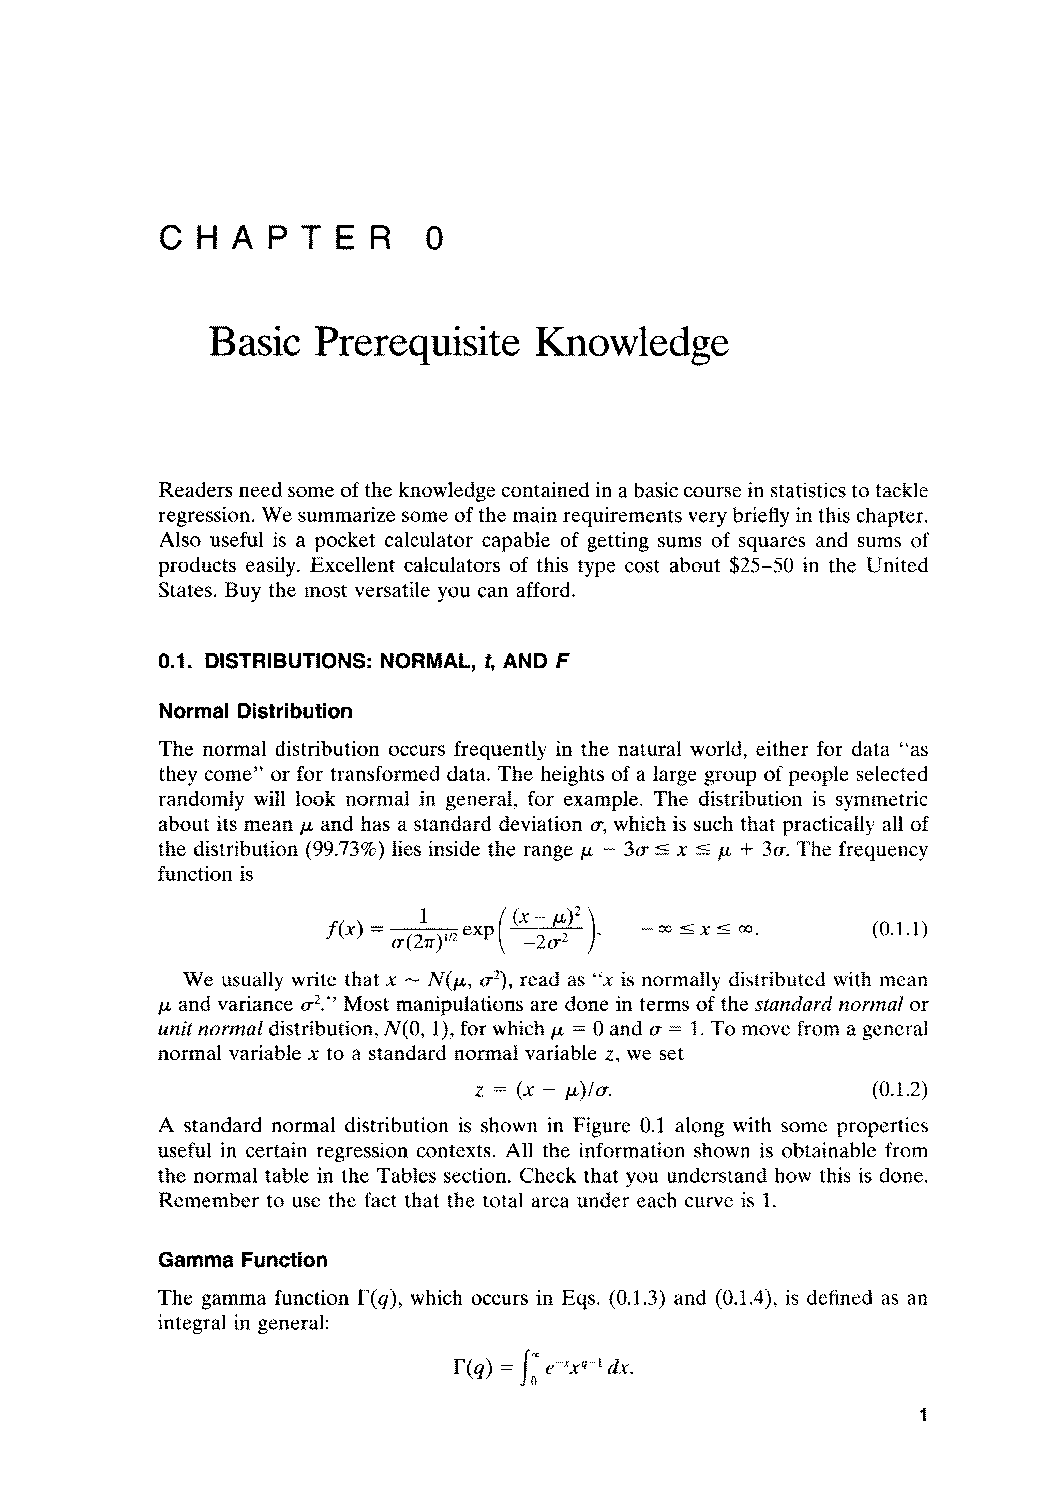
\includepdf[pages=-]{ch00.pdf}
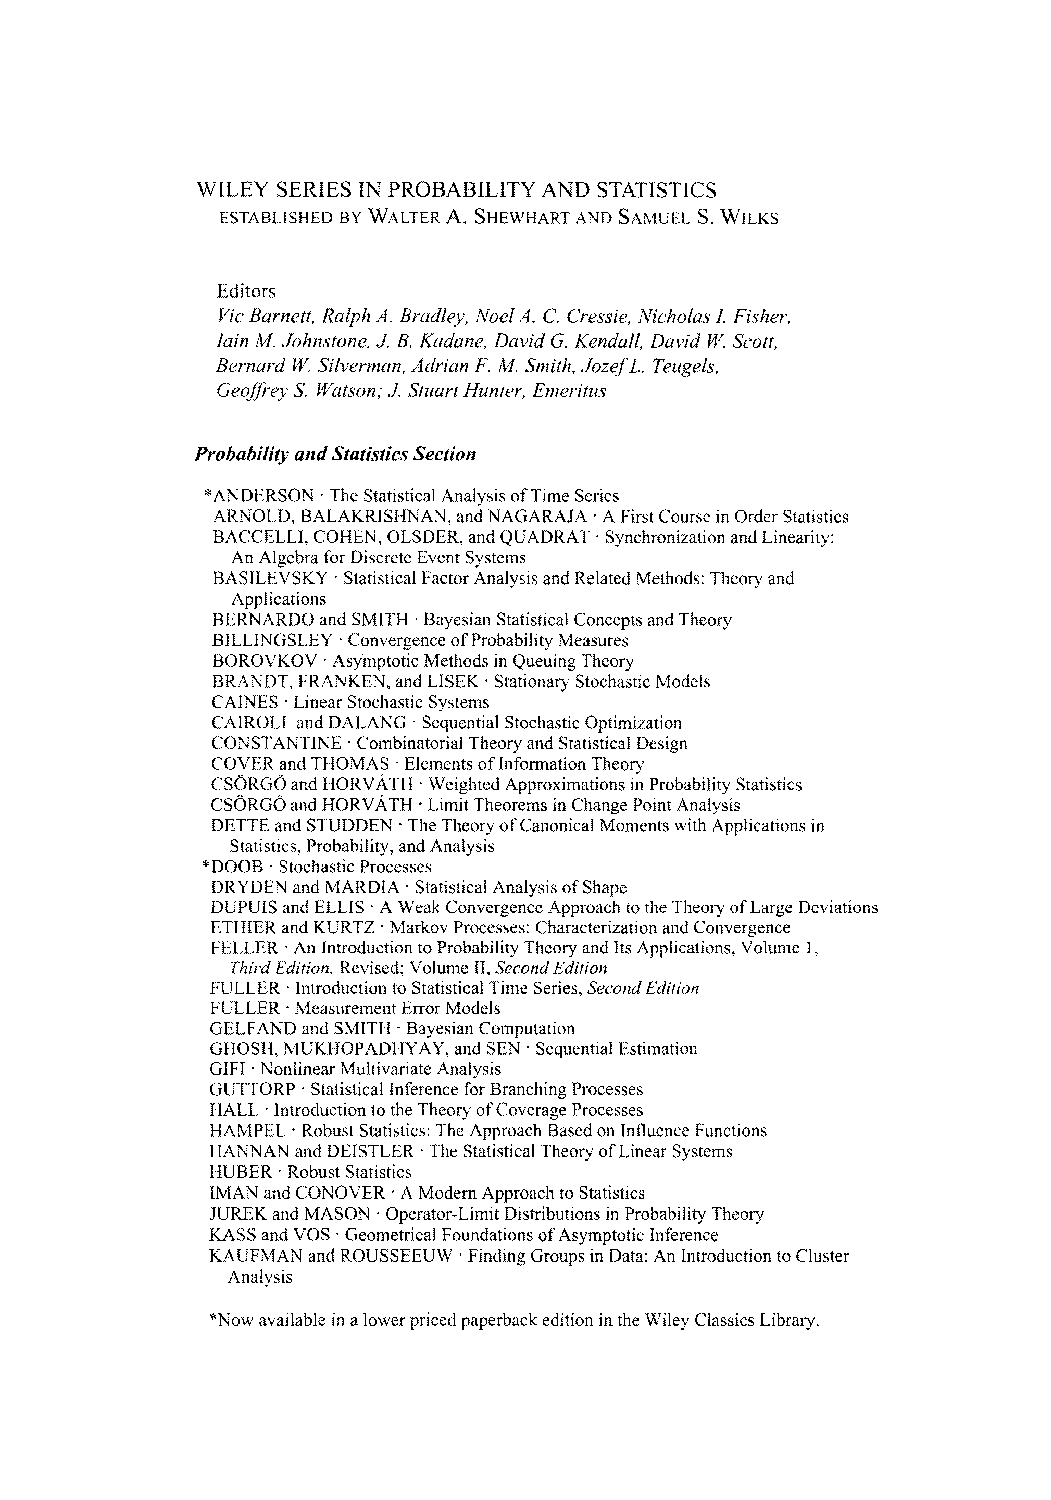
\includepdf[pages=-]{scard.pdf}
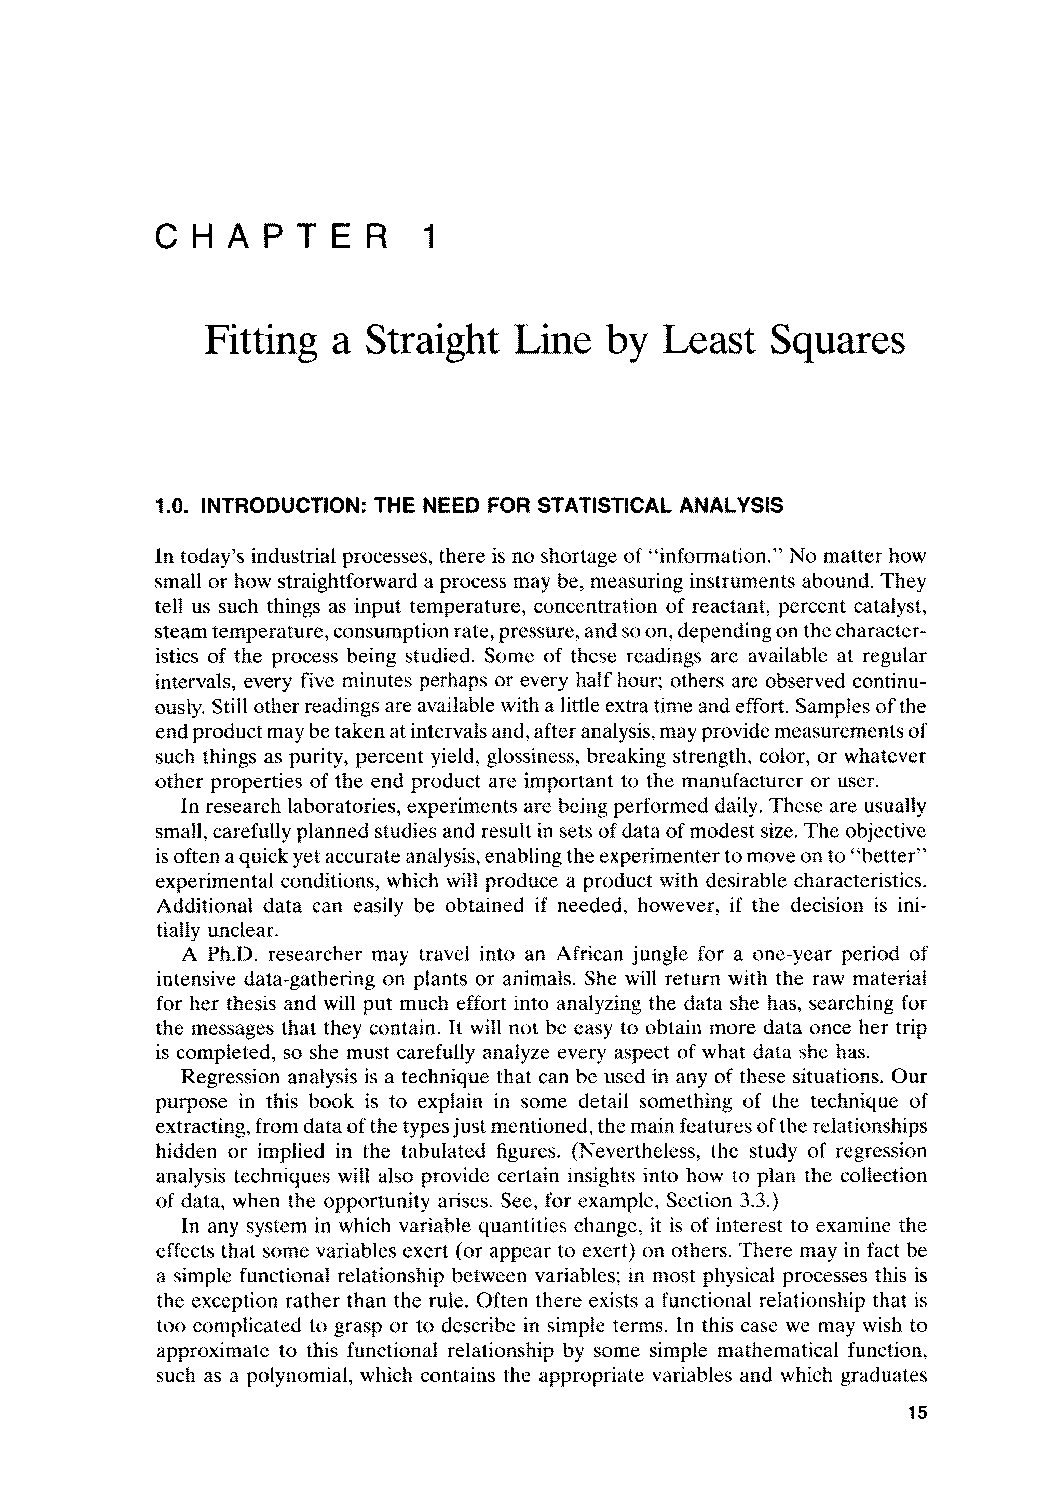
\includepdf[pages=-]{ch1.pdf}
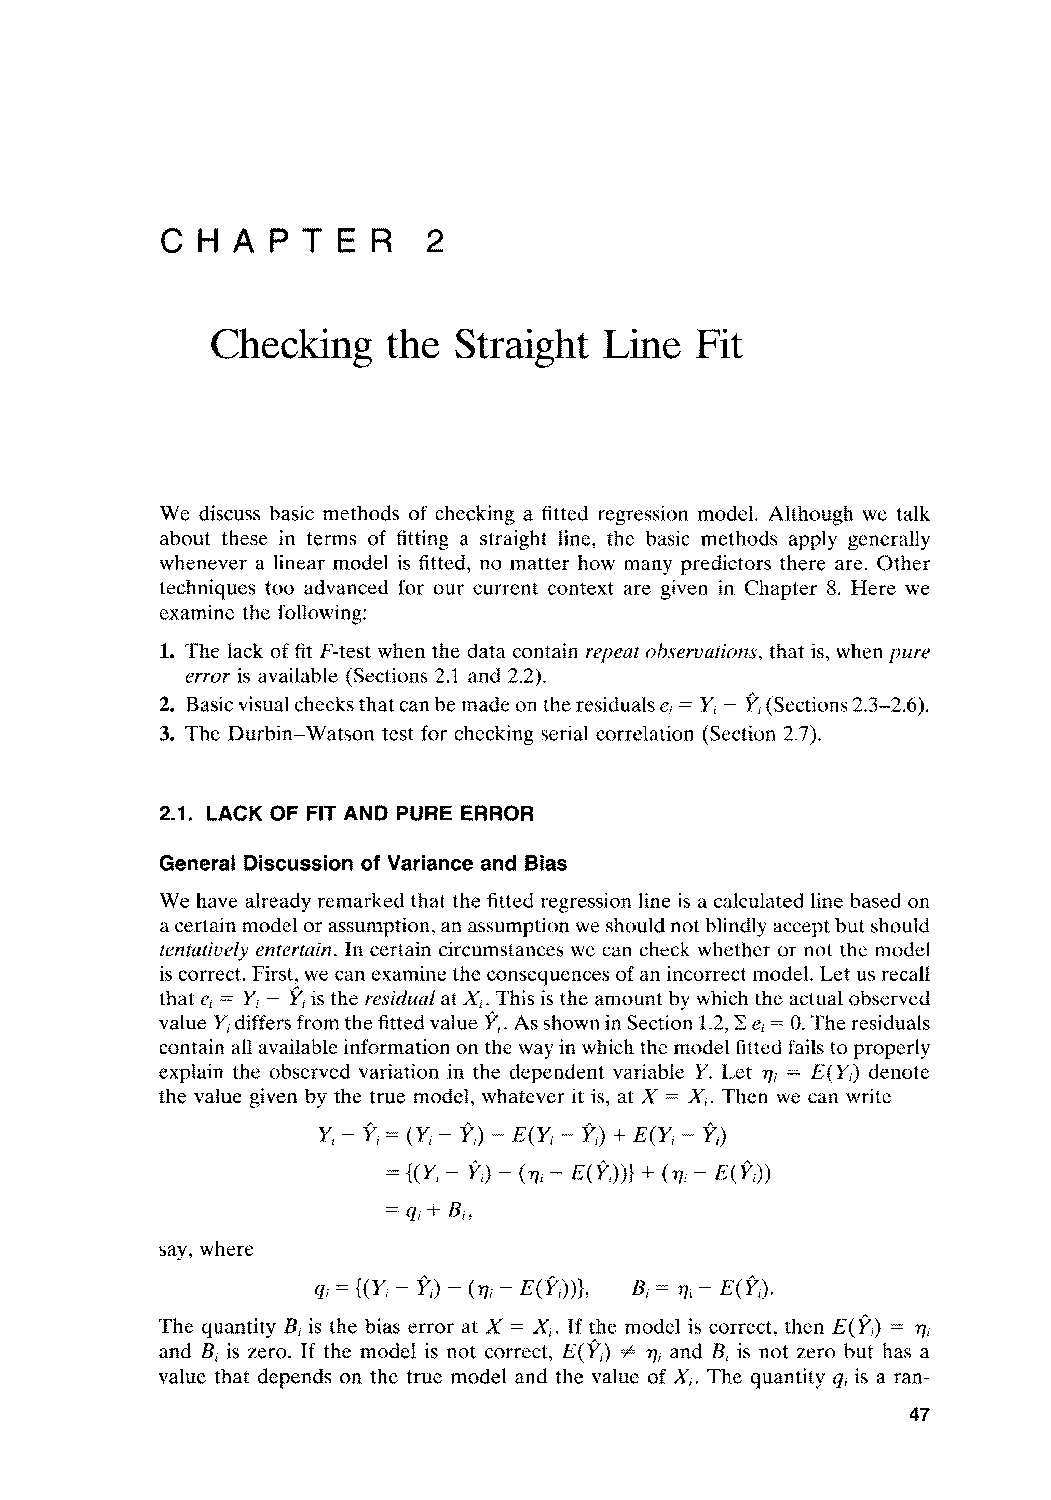
\includepdf[pages=-]{ch2.pdf}
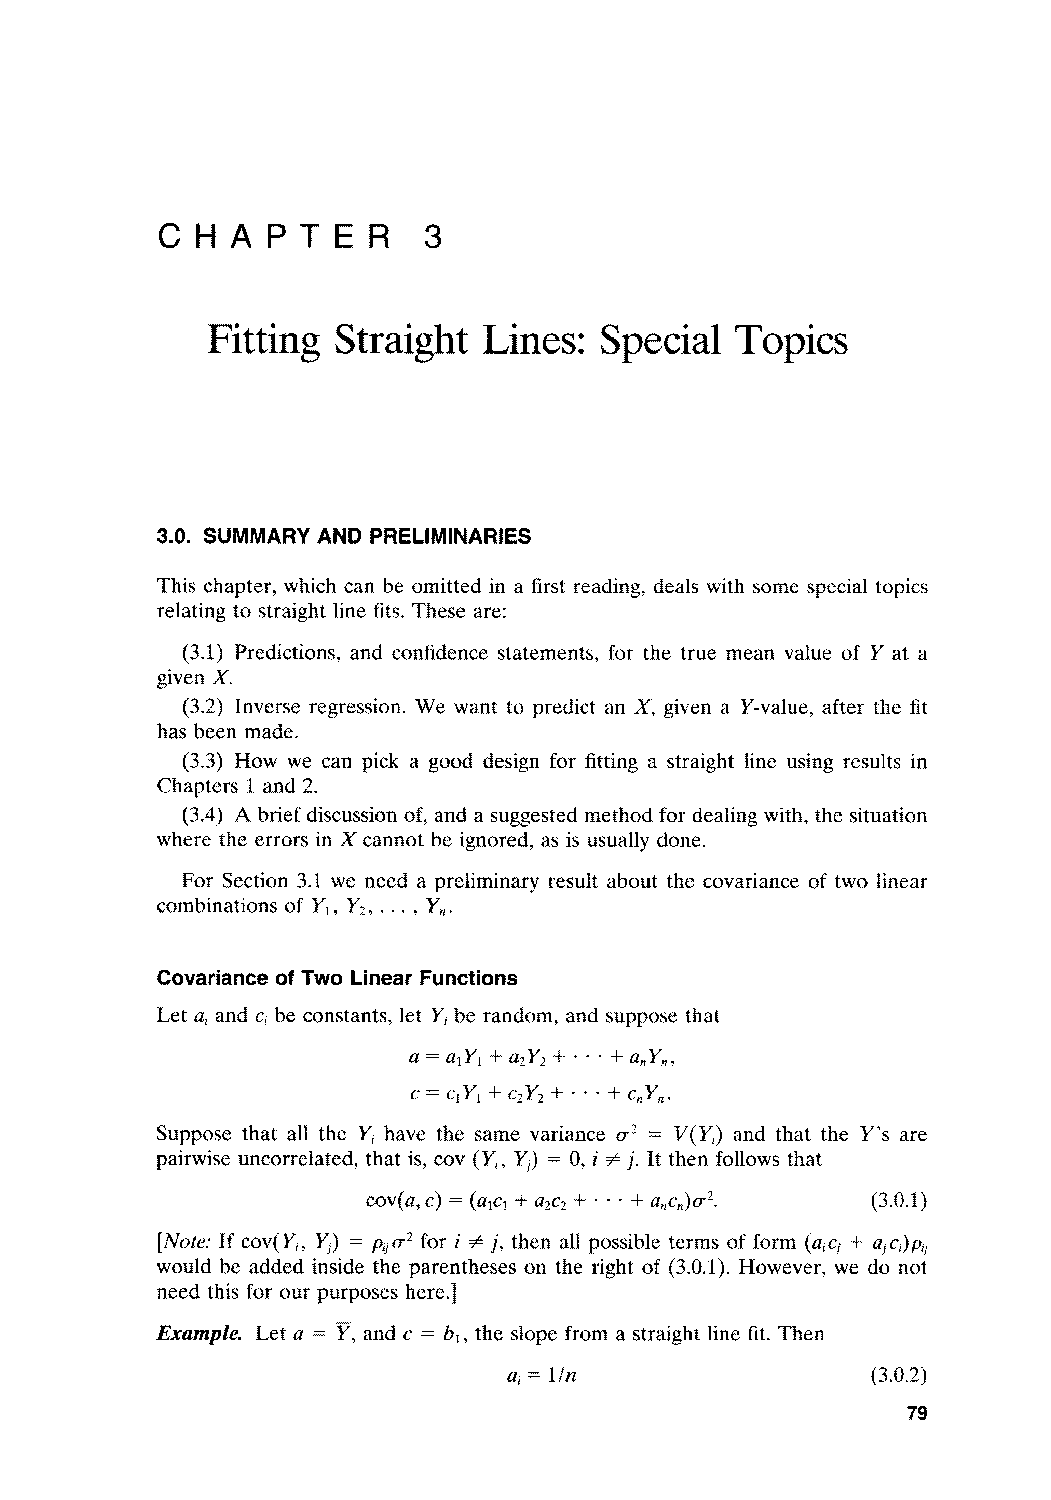
\includepdf[pages=-]{ch3.pdf}
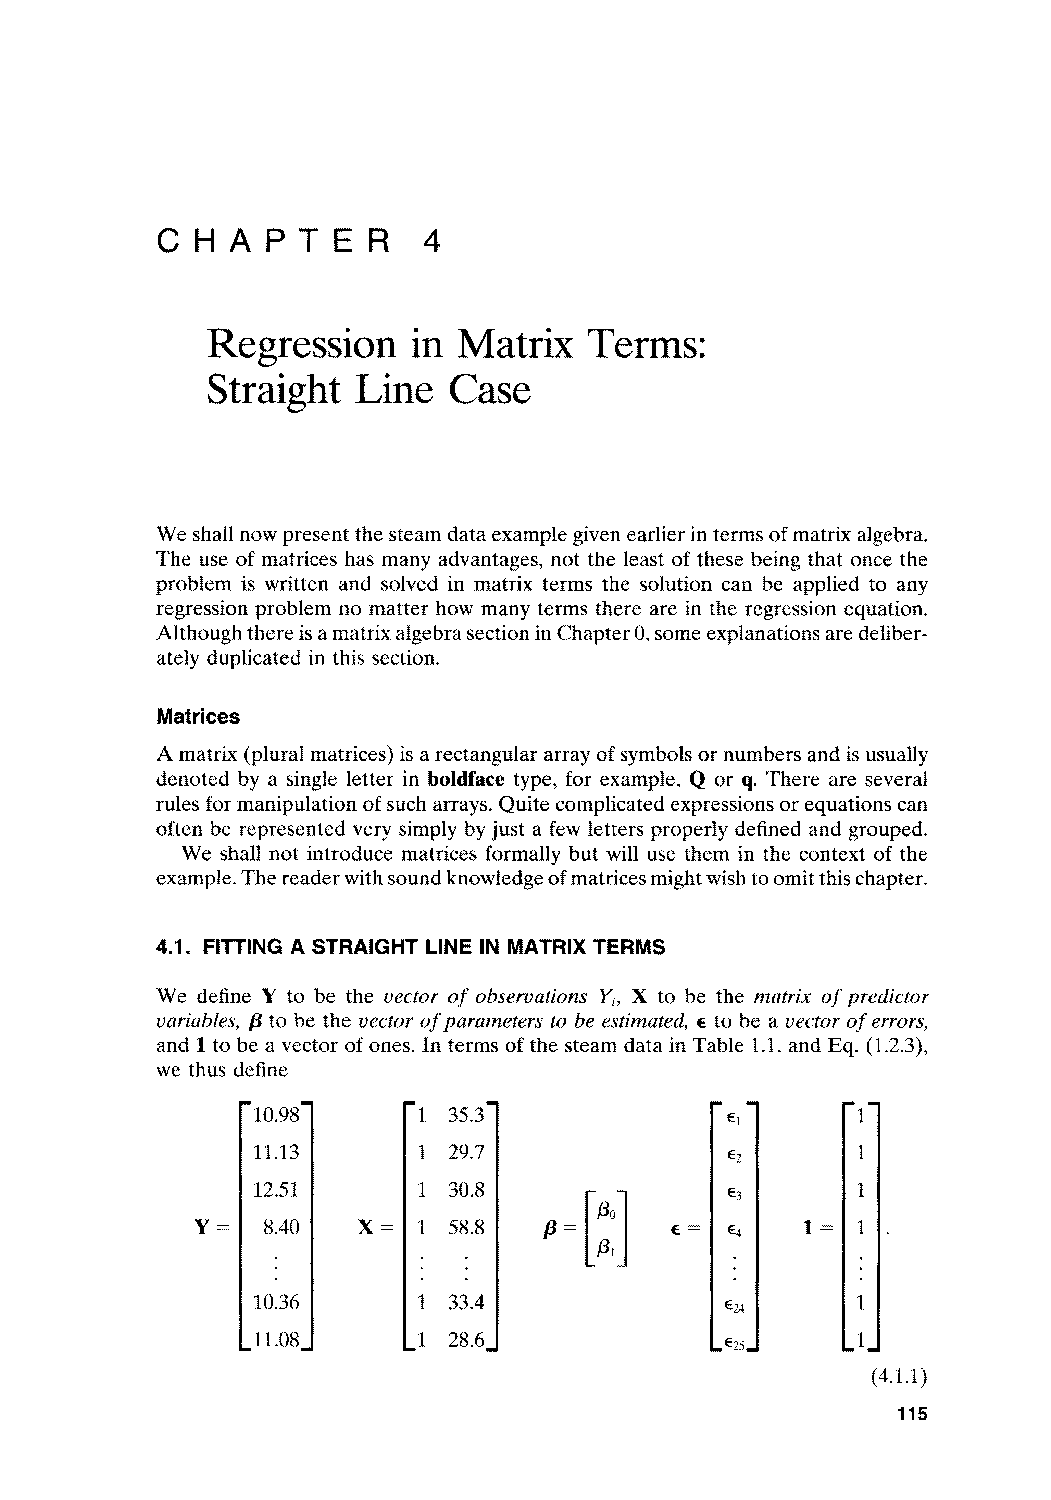
\includepdf[pages=-]{ch4.pdf}
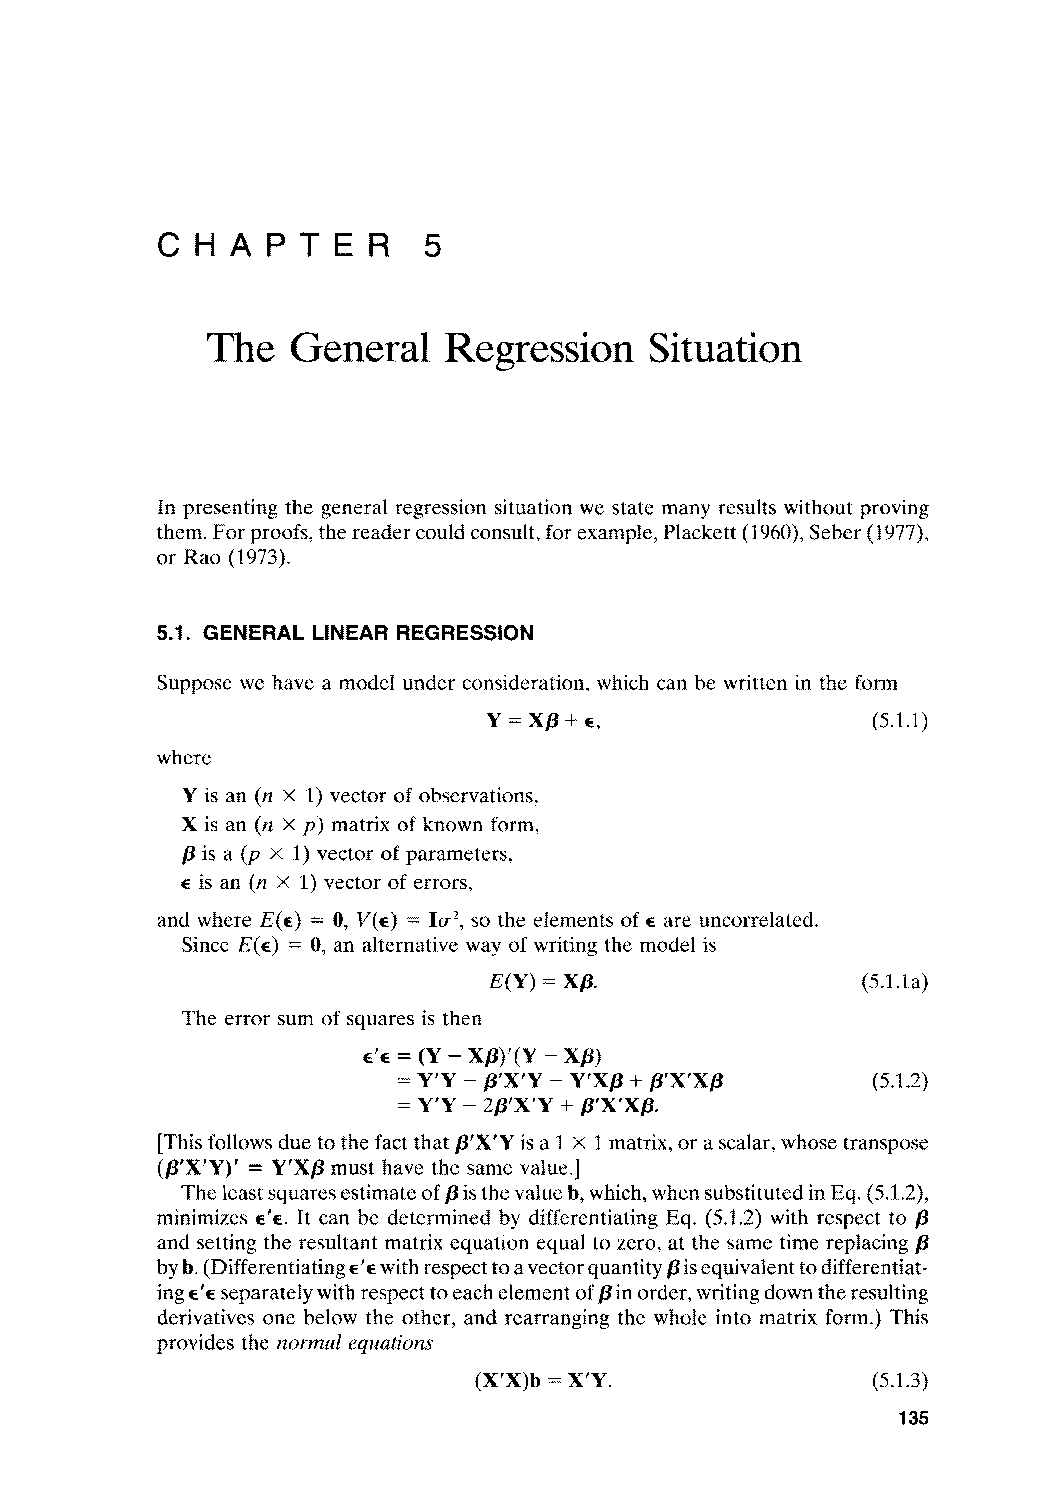
\includepdf[pages=-]{ch5.pdf}
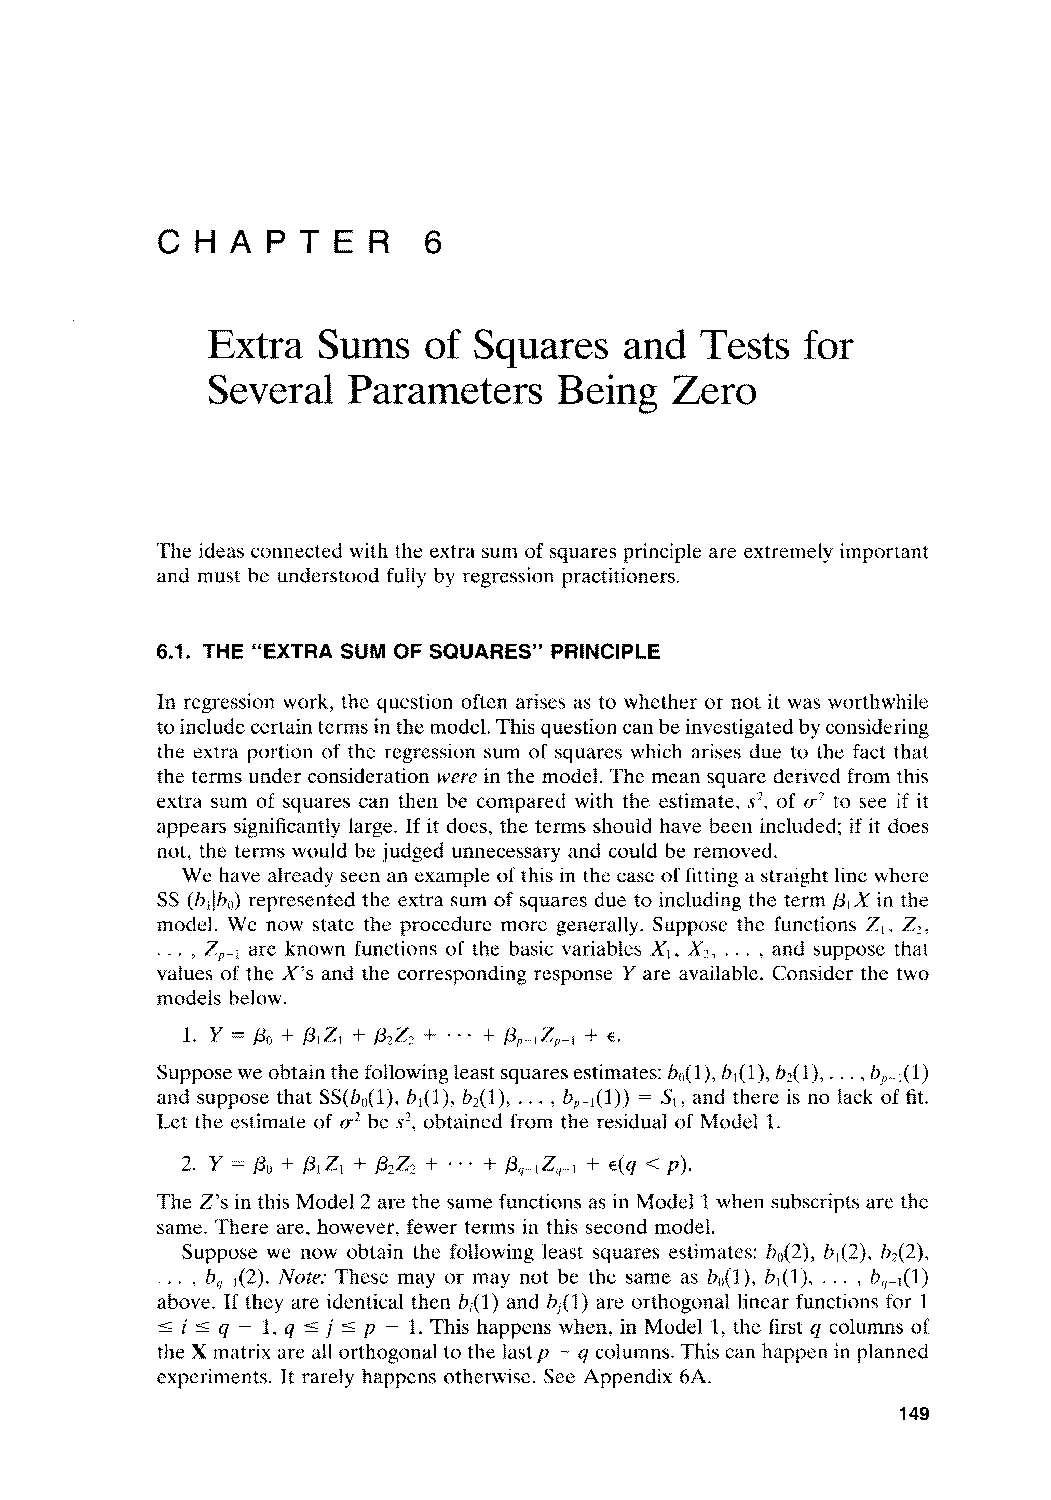
\includepdf[pages=-]{ch6.pdf}
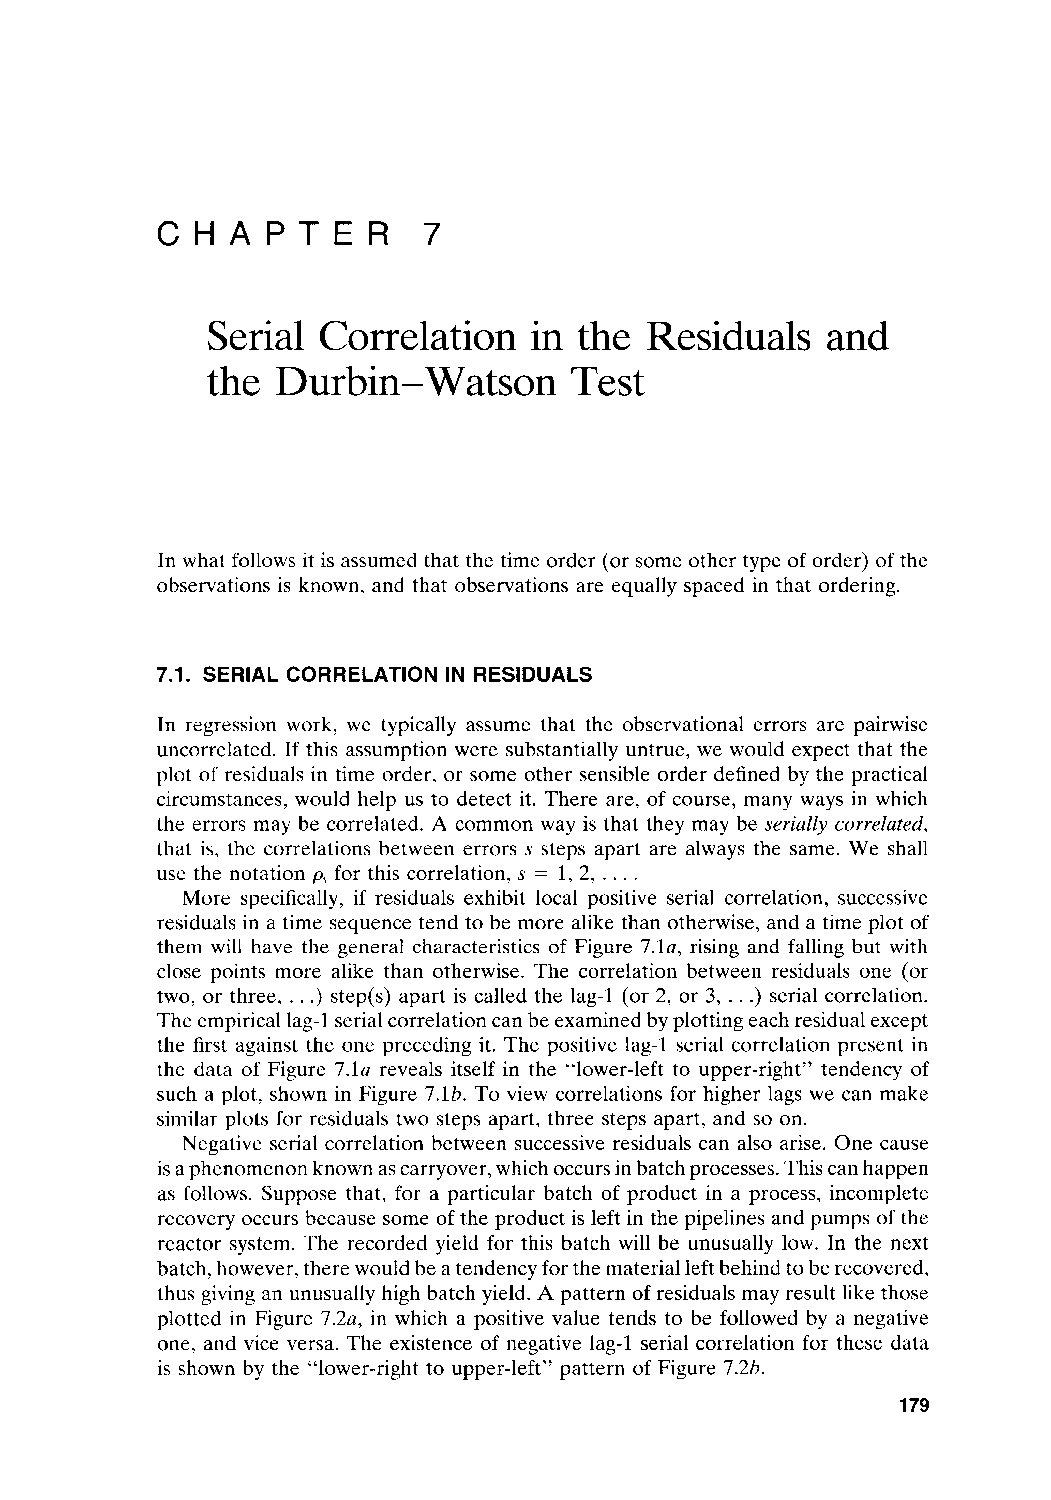
\includepdf[pages=-]{ch7.pdf}
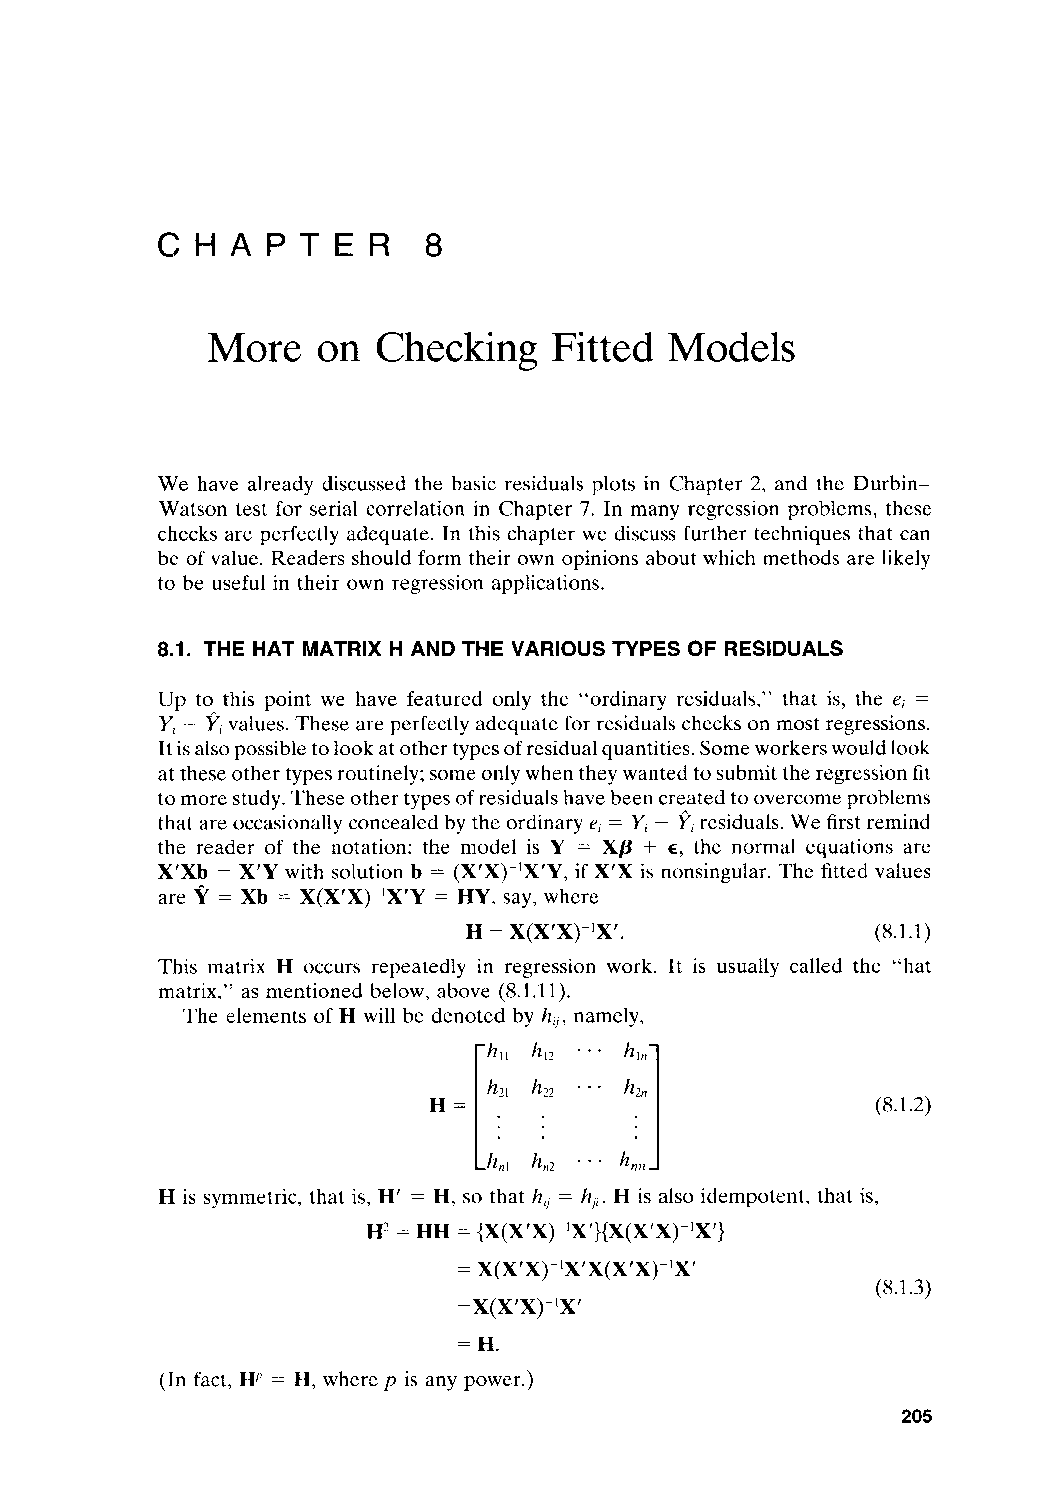
\includepdf[pages=-]{ch8.pdf}
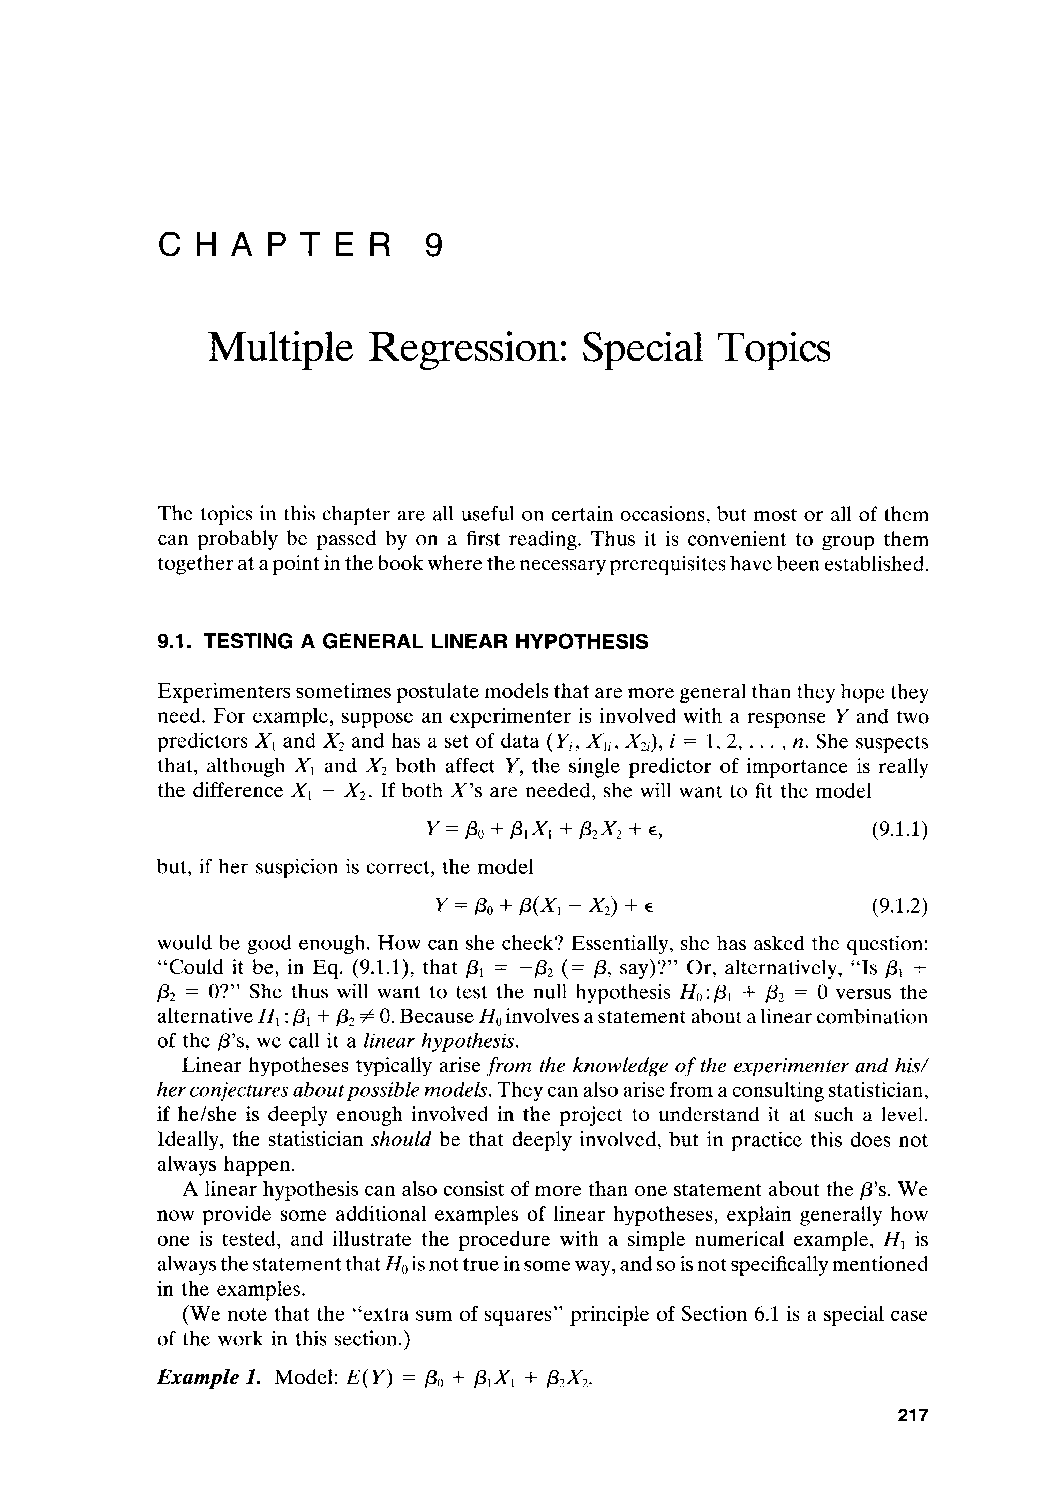
\includepdf[pages=-]{ch9.pdf}
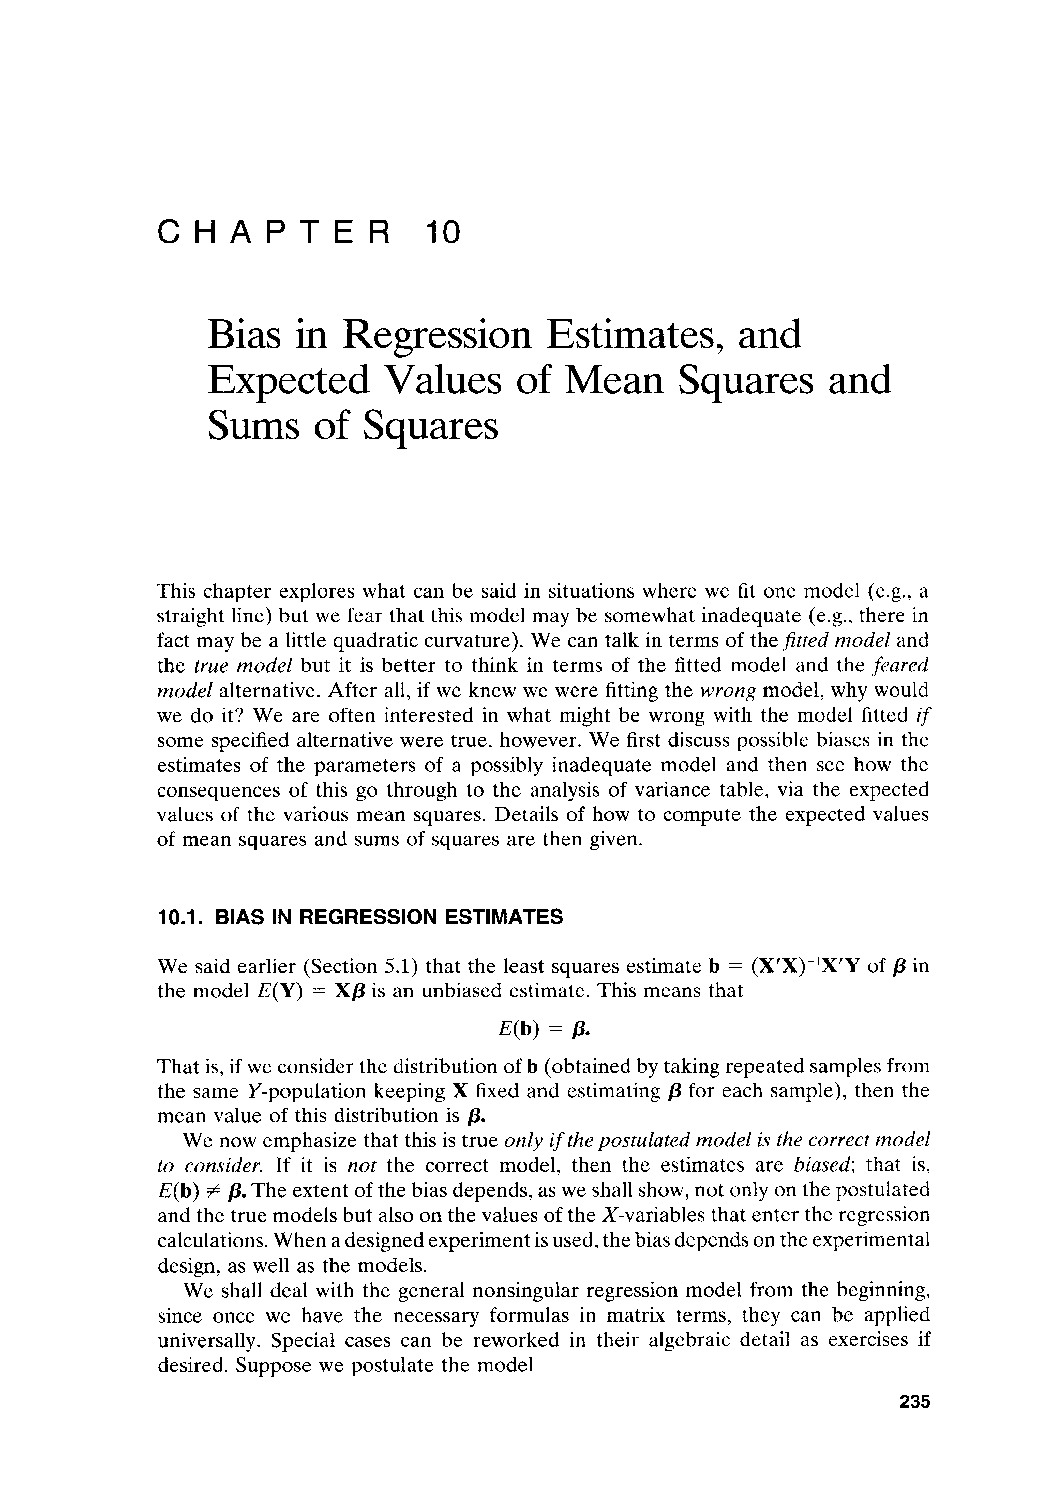
\includepdf[pages=-]{ch10.pdf}
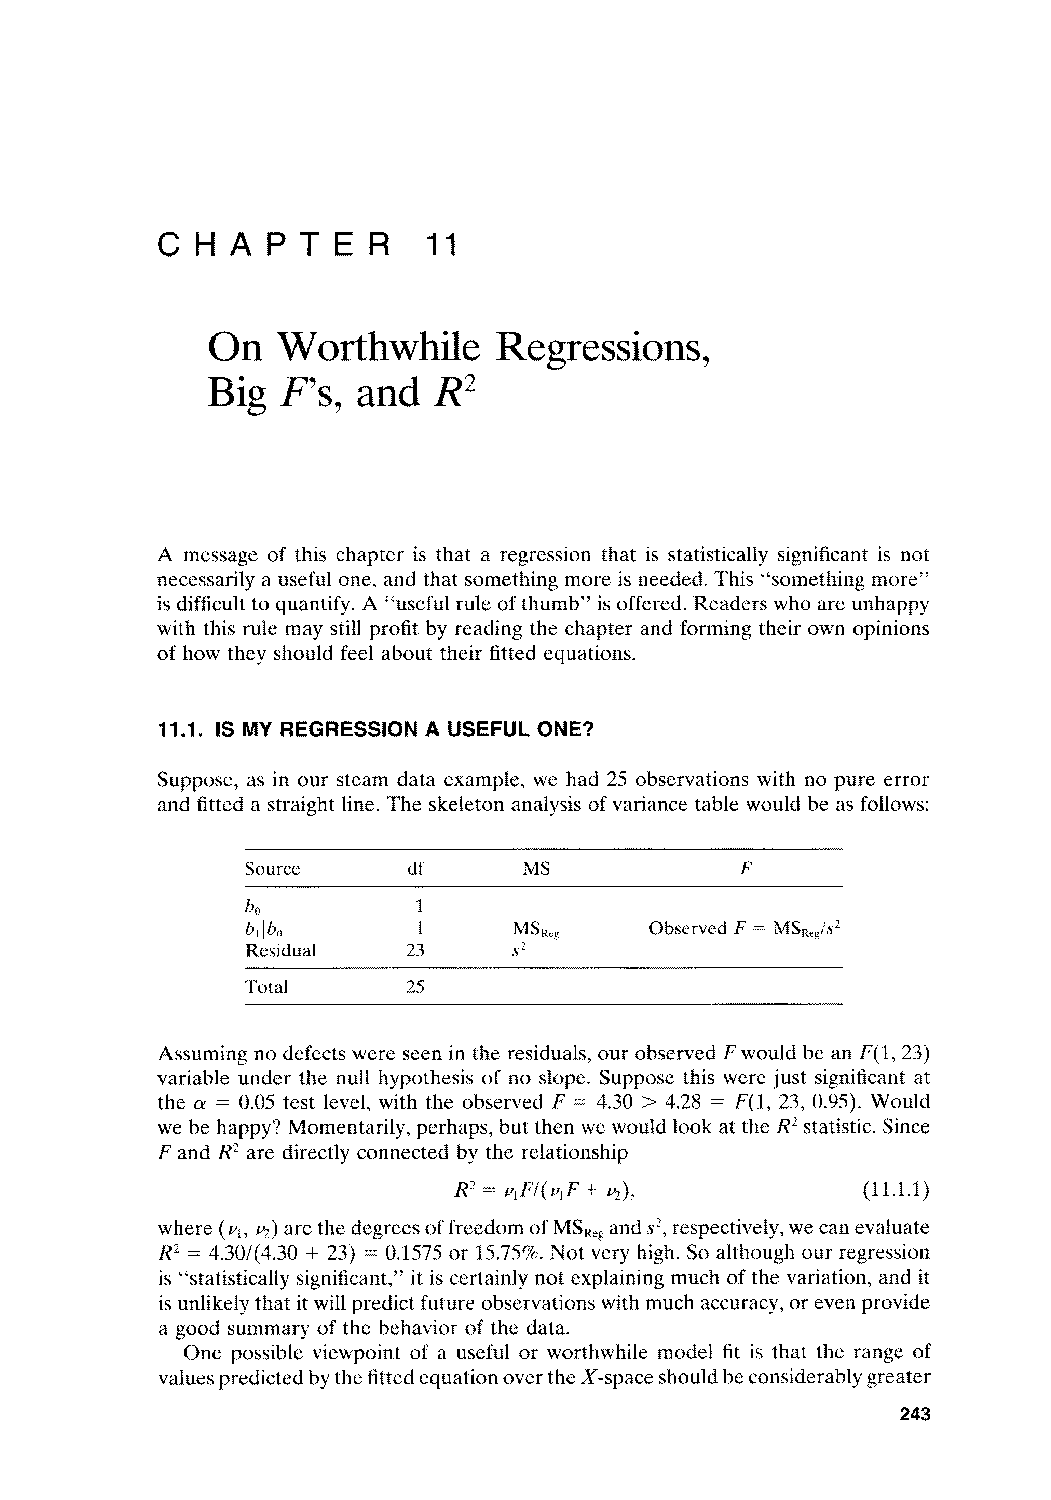
\includepdf[pages=-]{ch11.pdf}
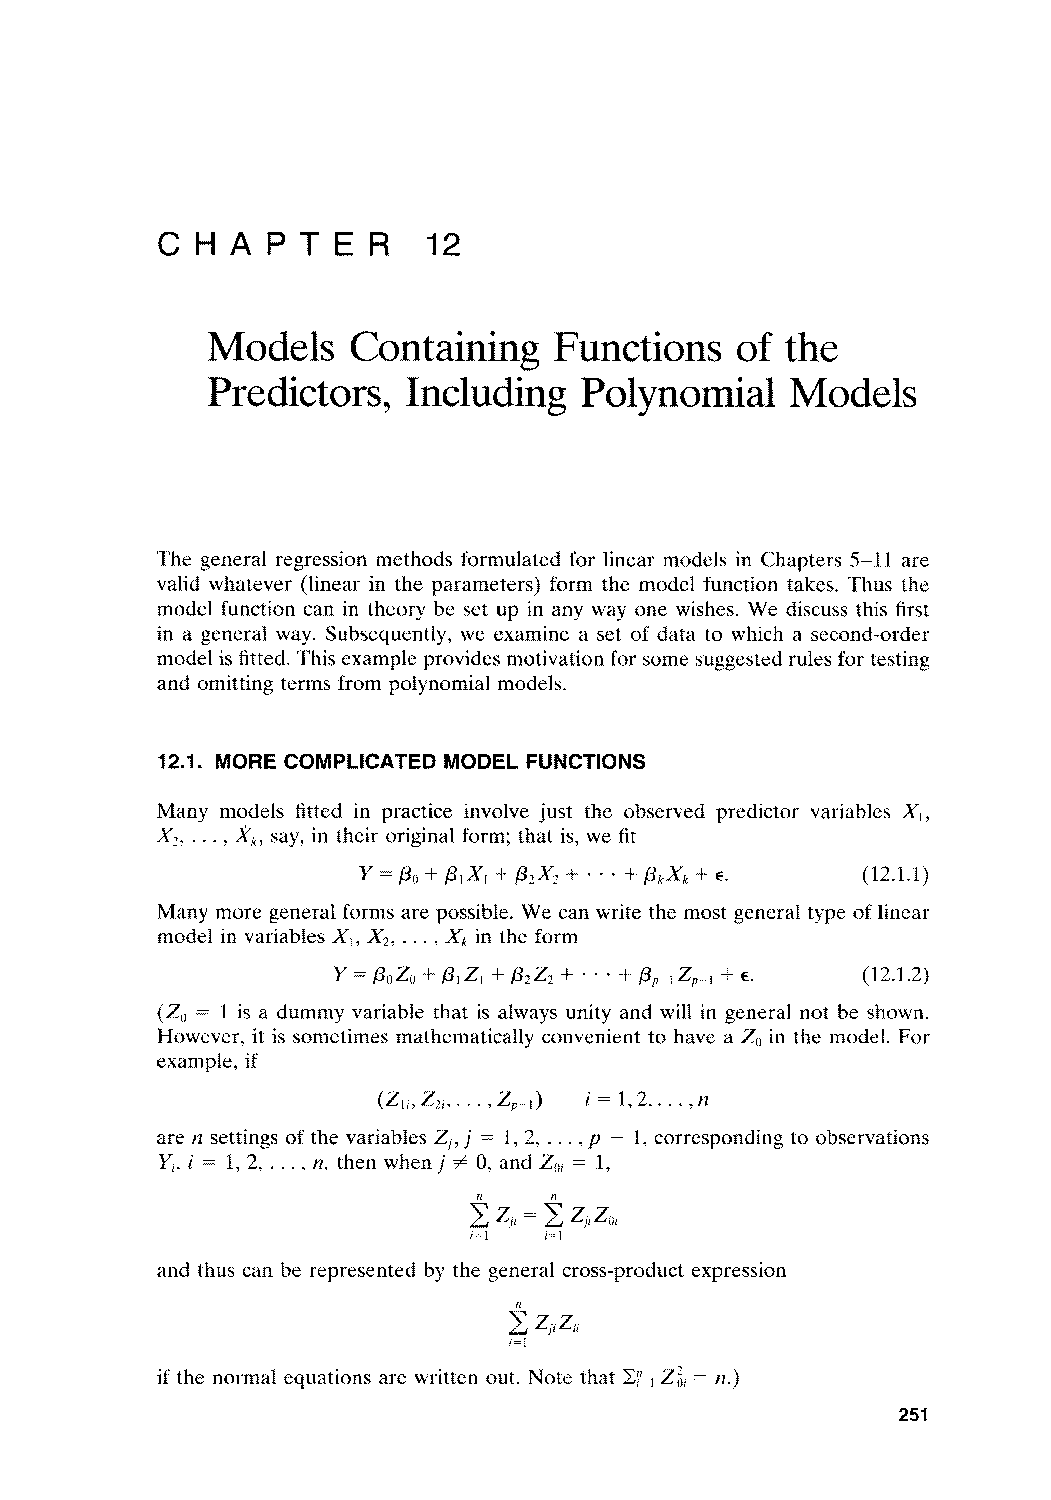
\includepdf[pages=-]{ch12.pdf}
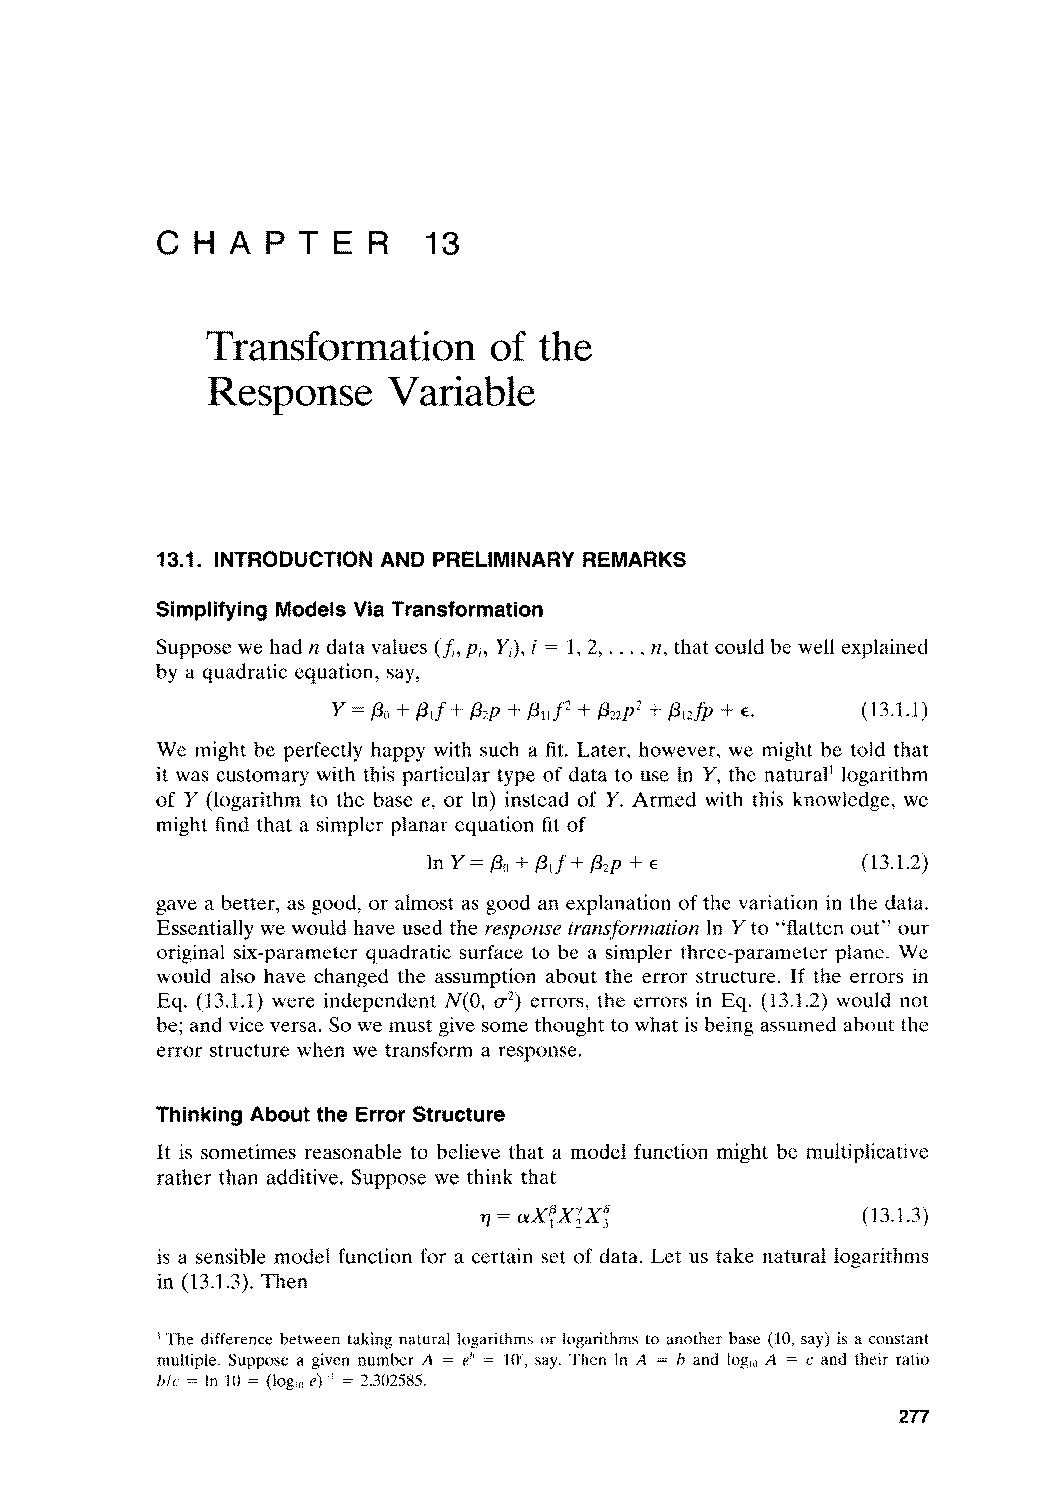
\includepdf[pages=-]{ch13.pdf}
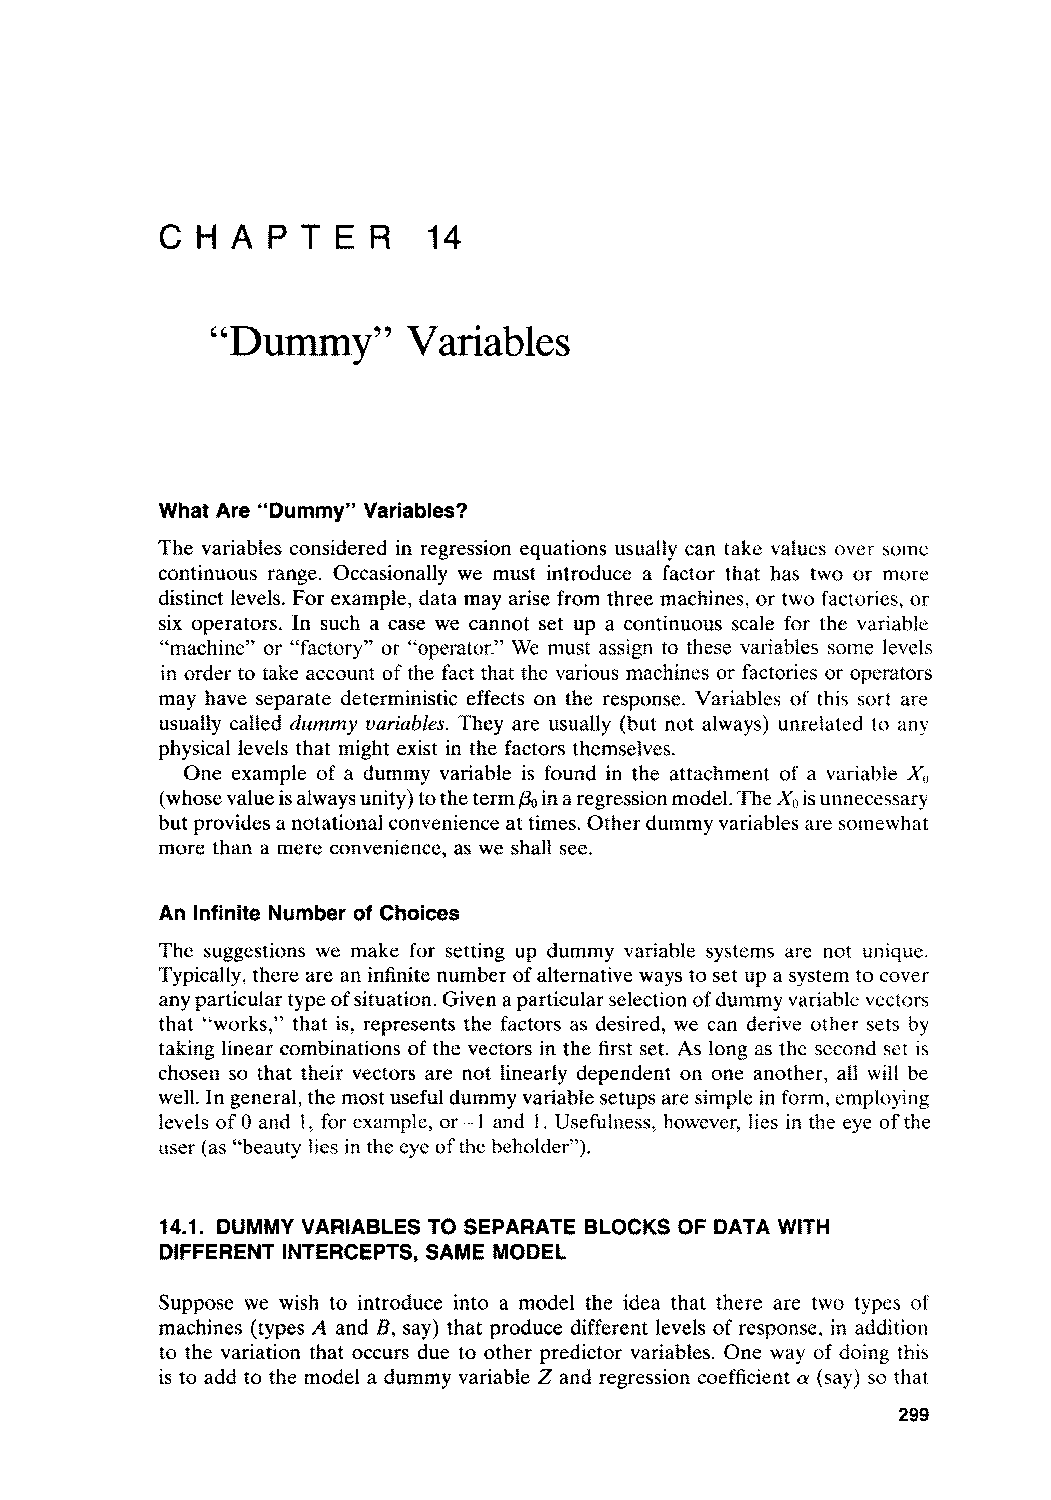
\includepdf[pages=-]{ch14.pdf}
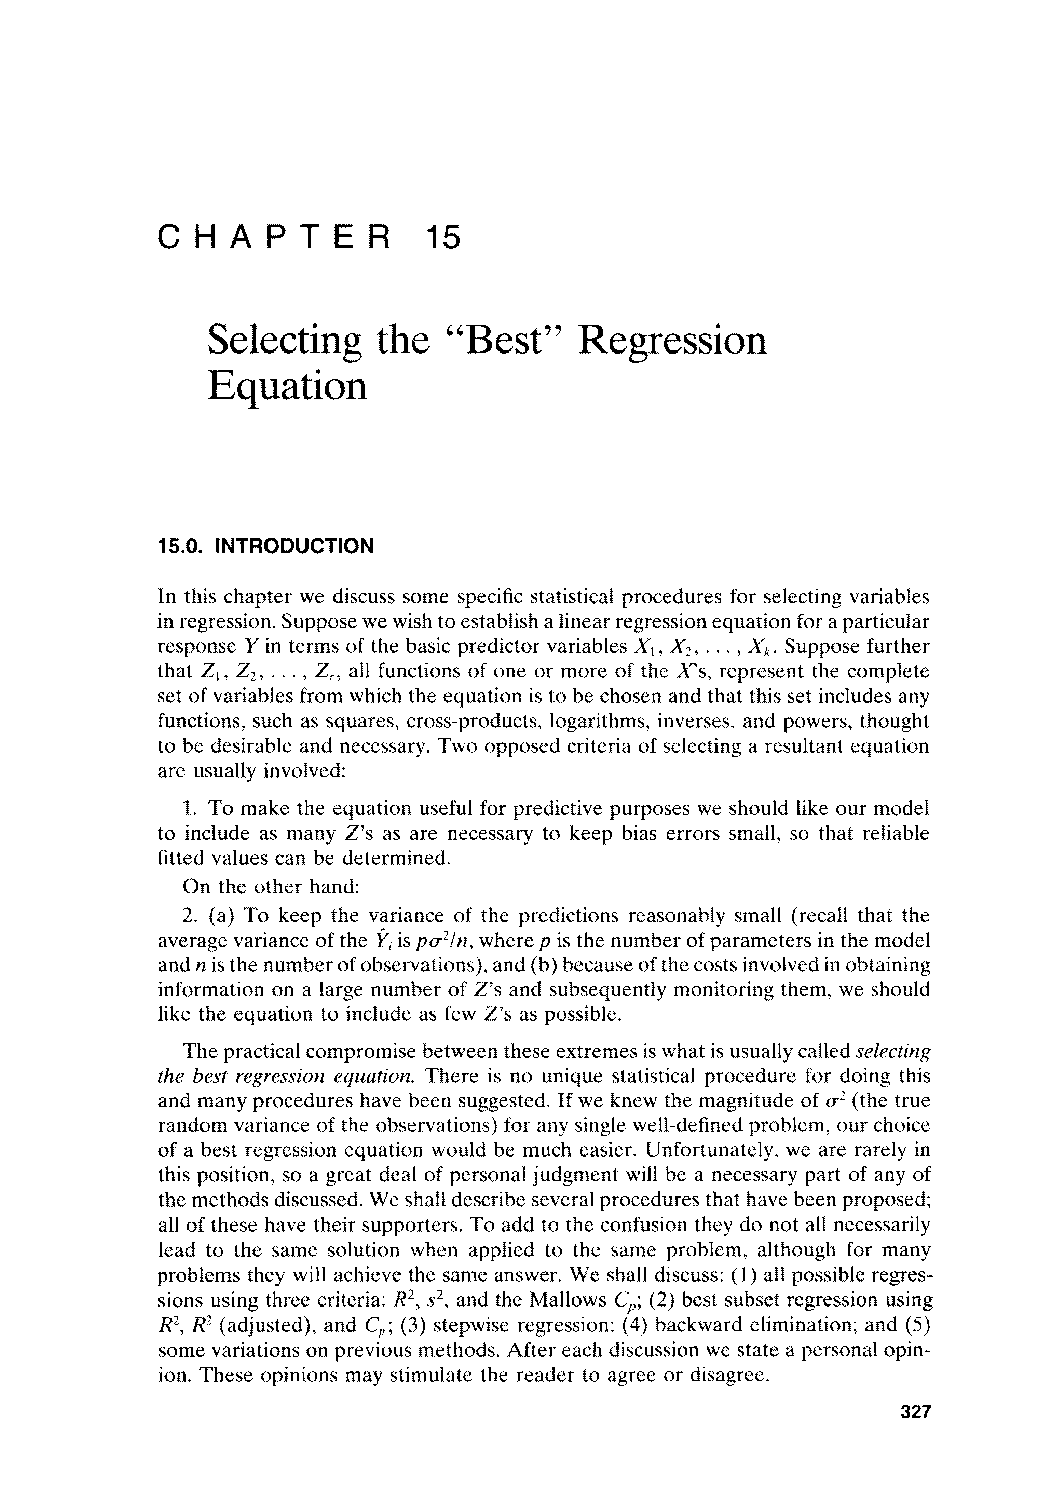
\includepdf[pages=-]{ch15.pdf}
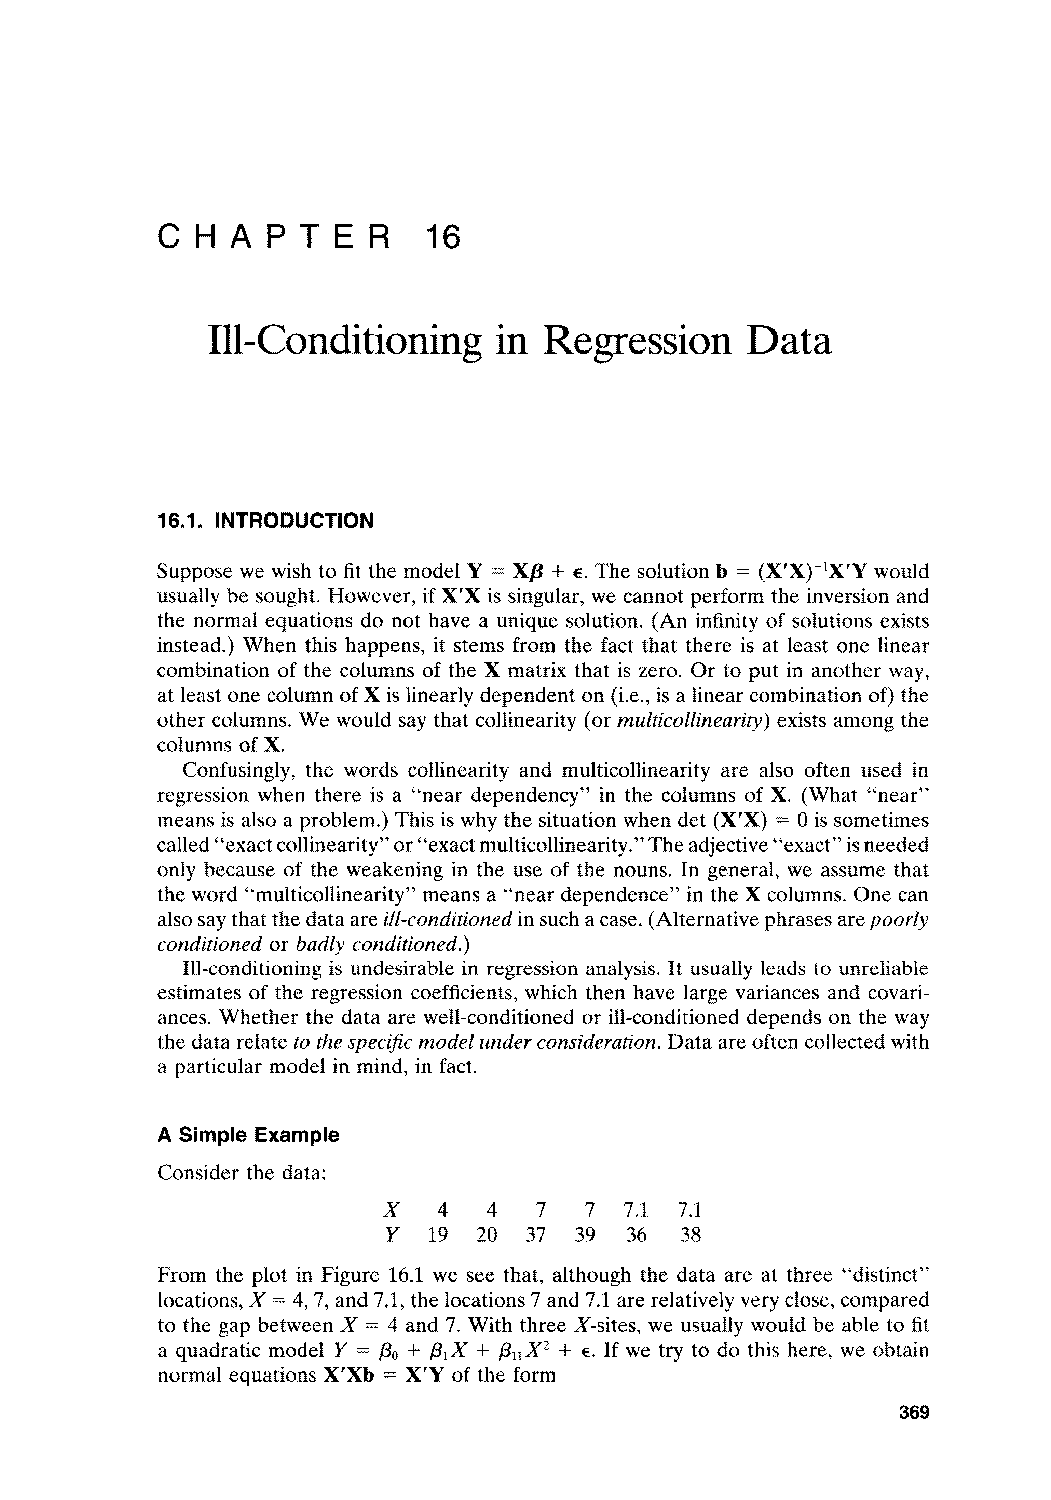
\includepdf[pages=-]{ch16.pdf}
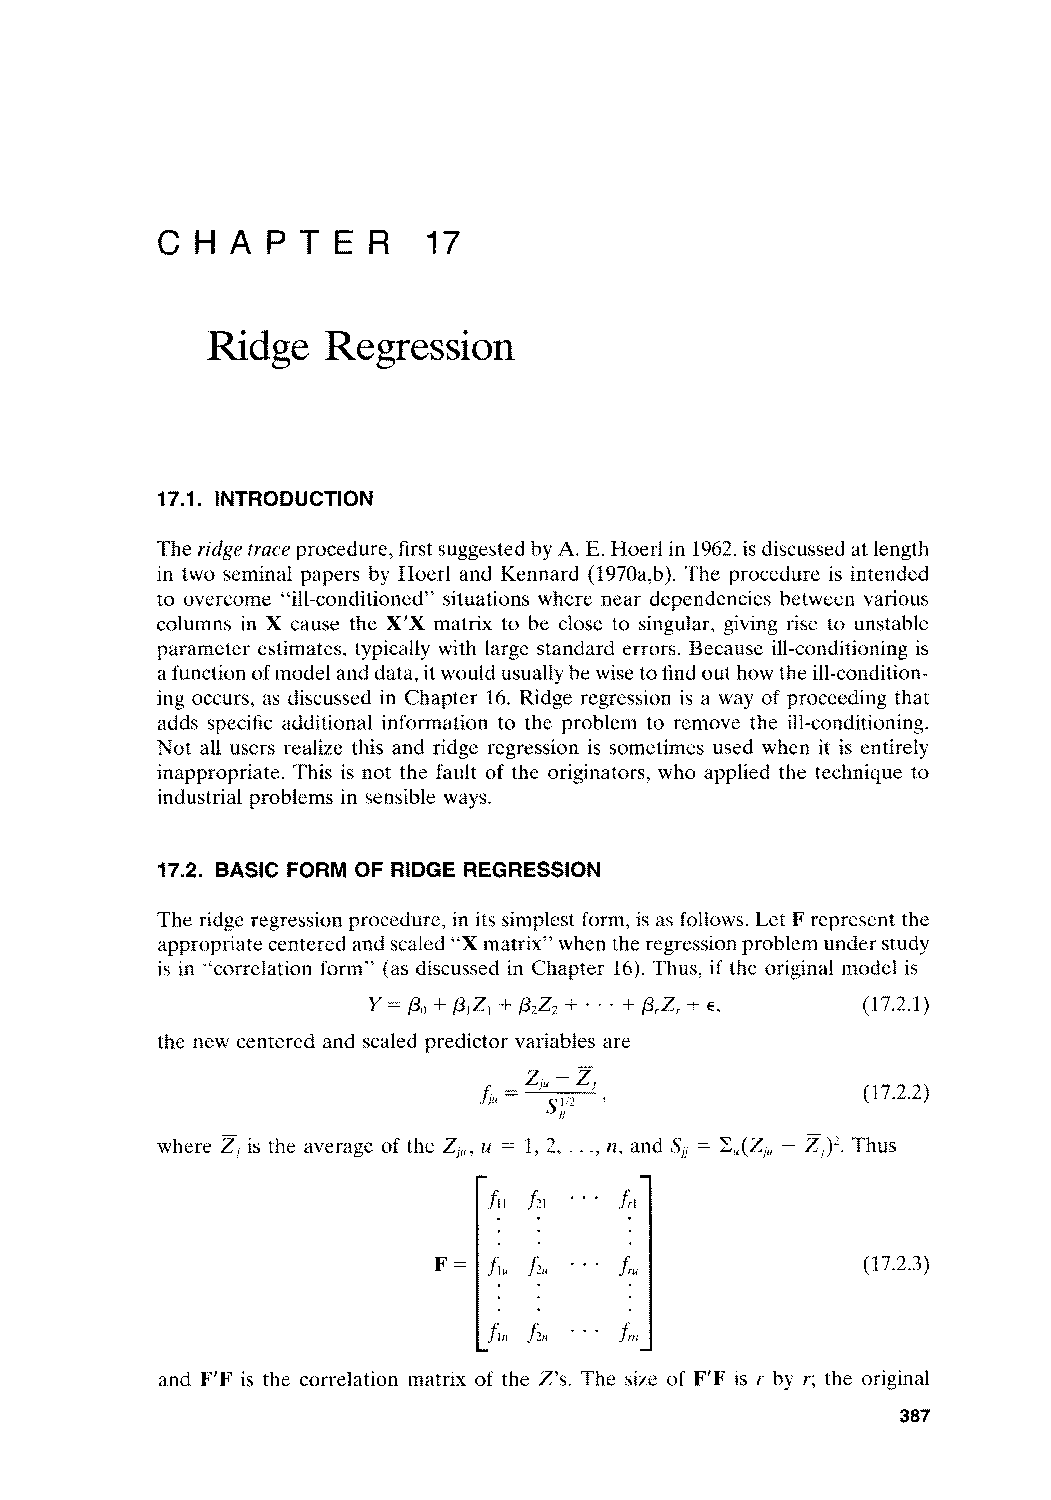
\includepdf[pages=-]{ch17.pdf}
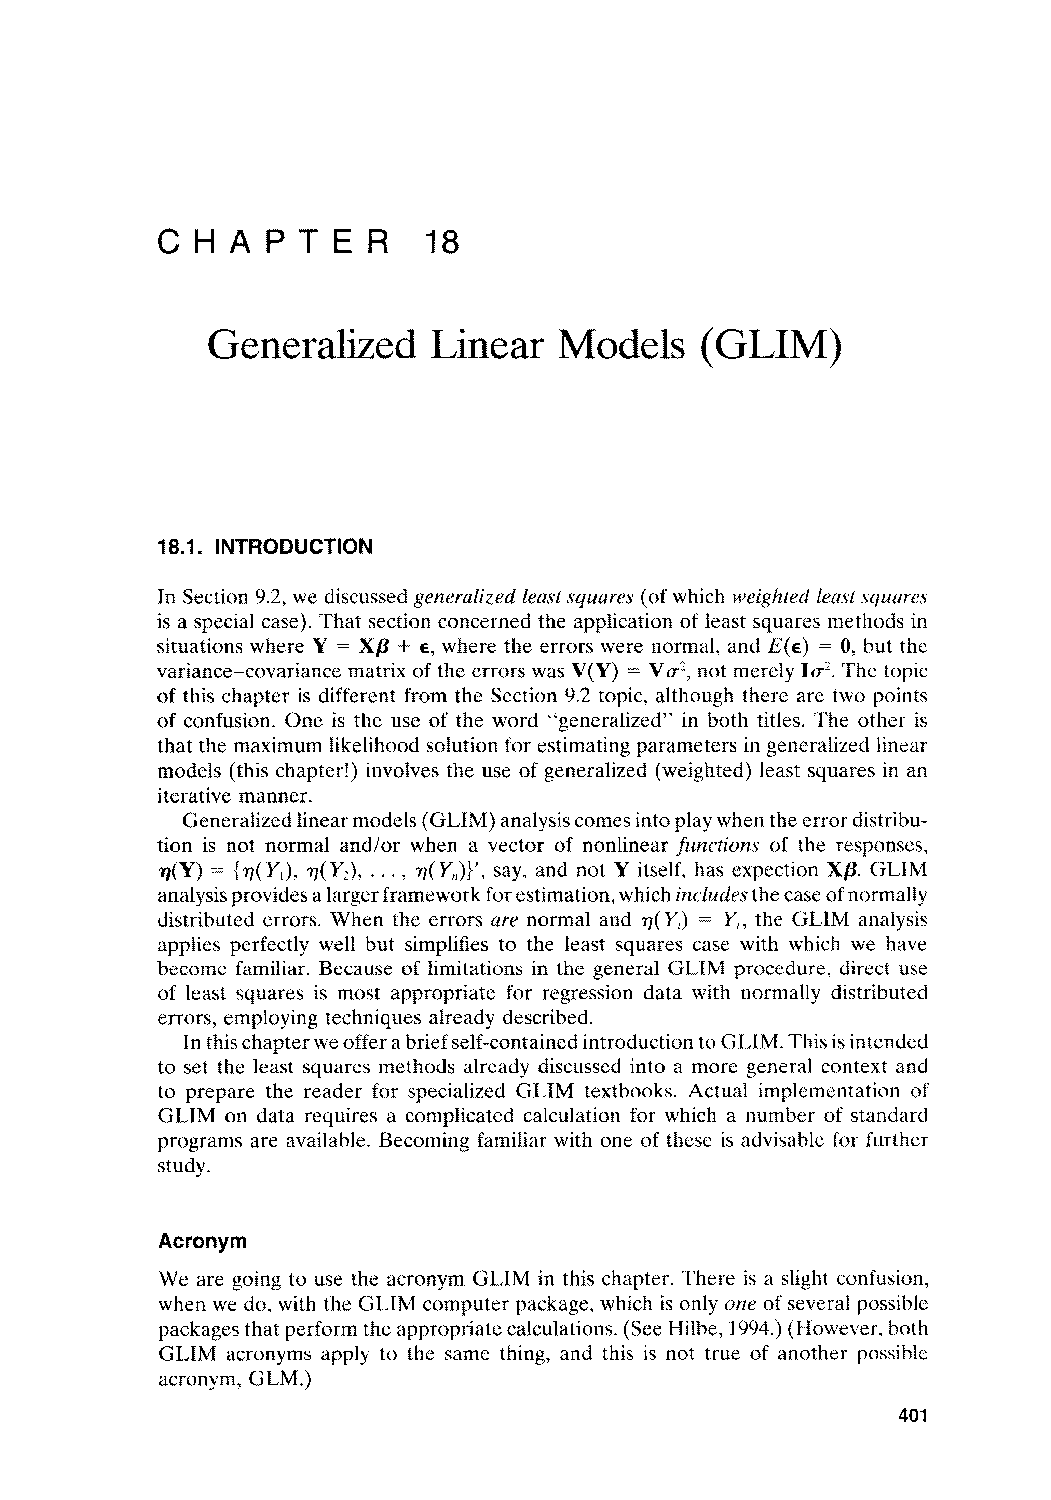
\includepdf[pages=-]{ch18.pdf}
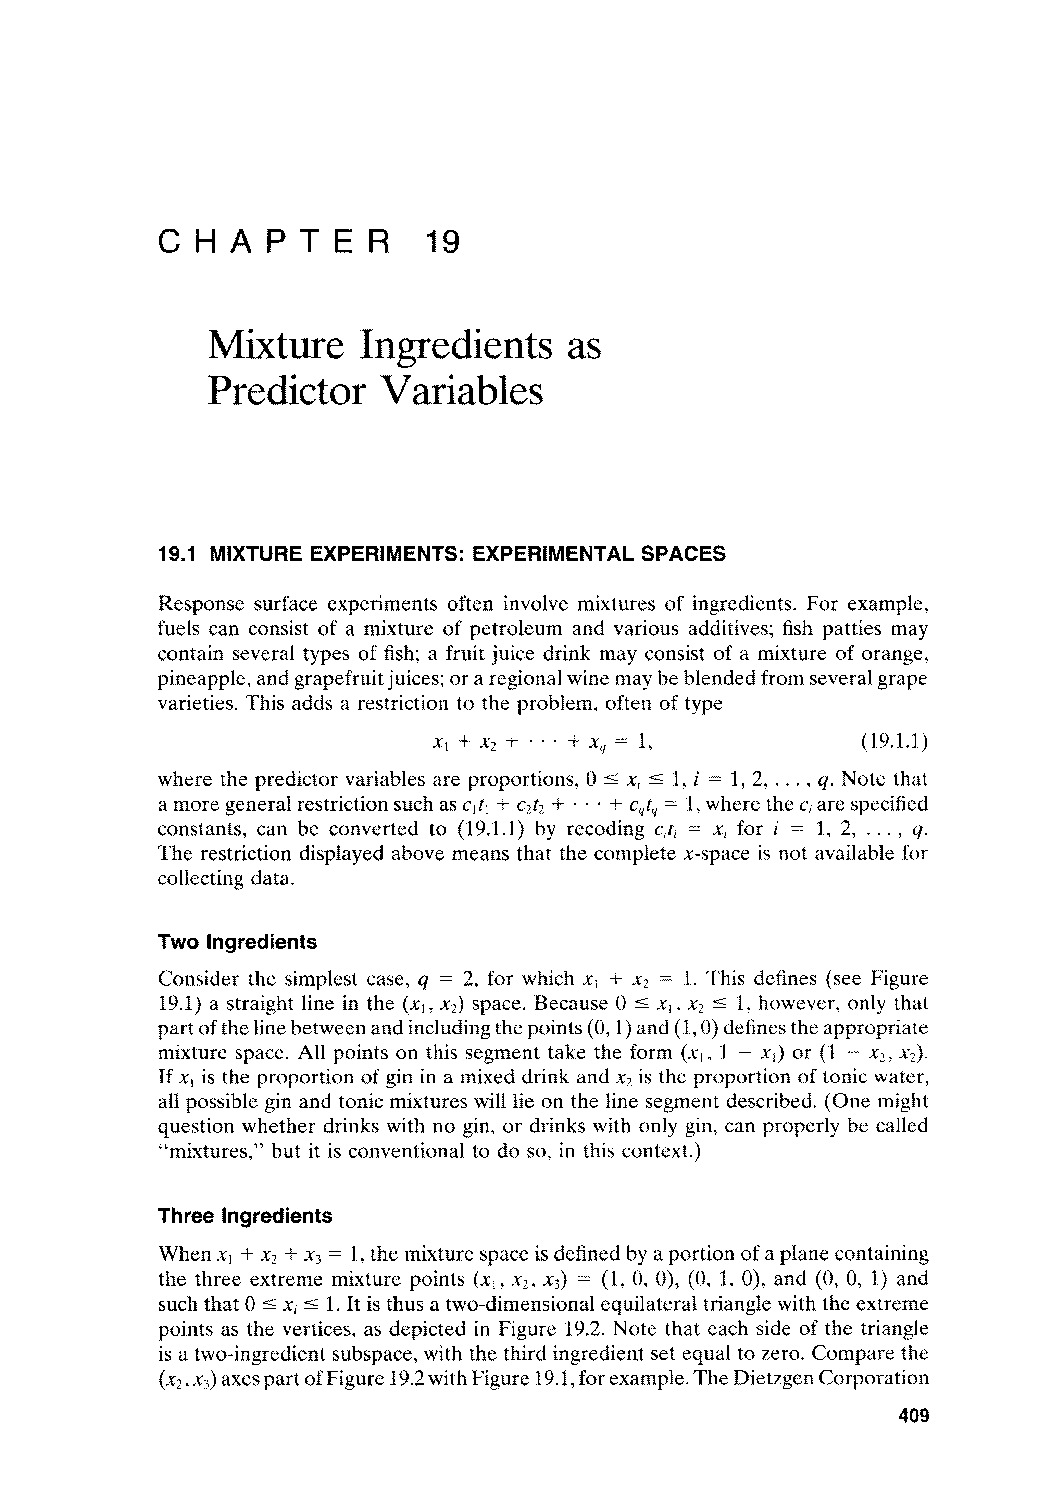
\includepdf[pages=-]{ch19.pdf}
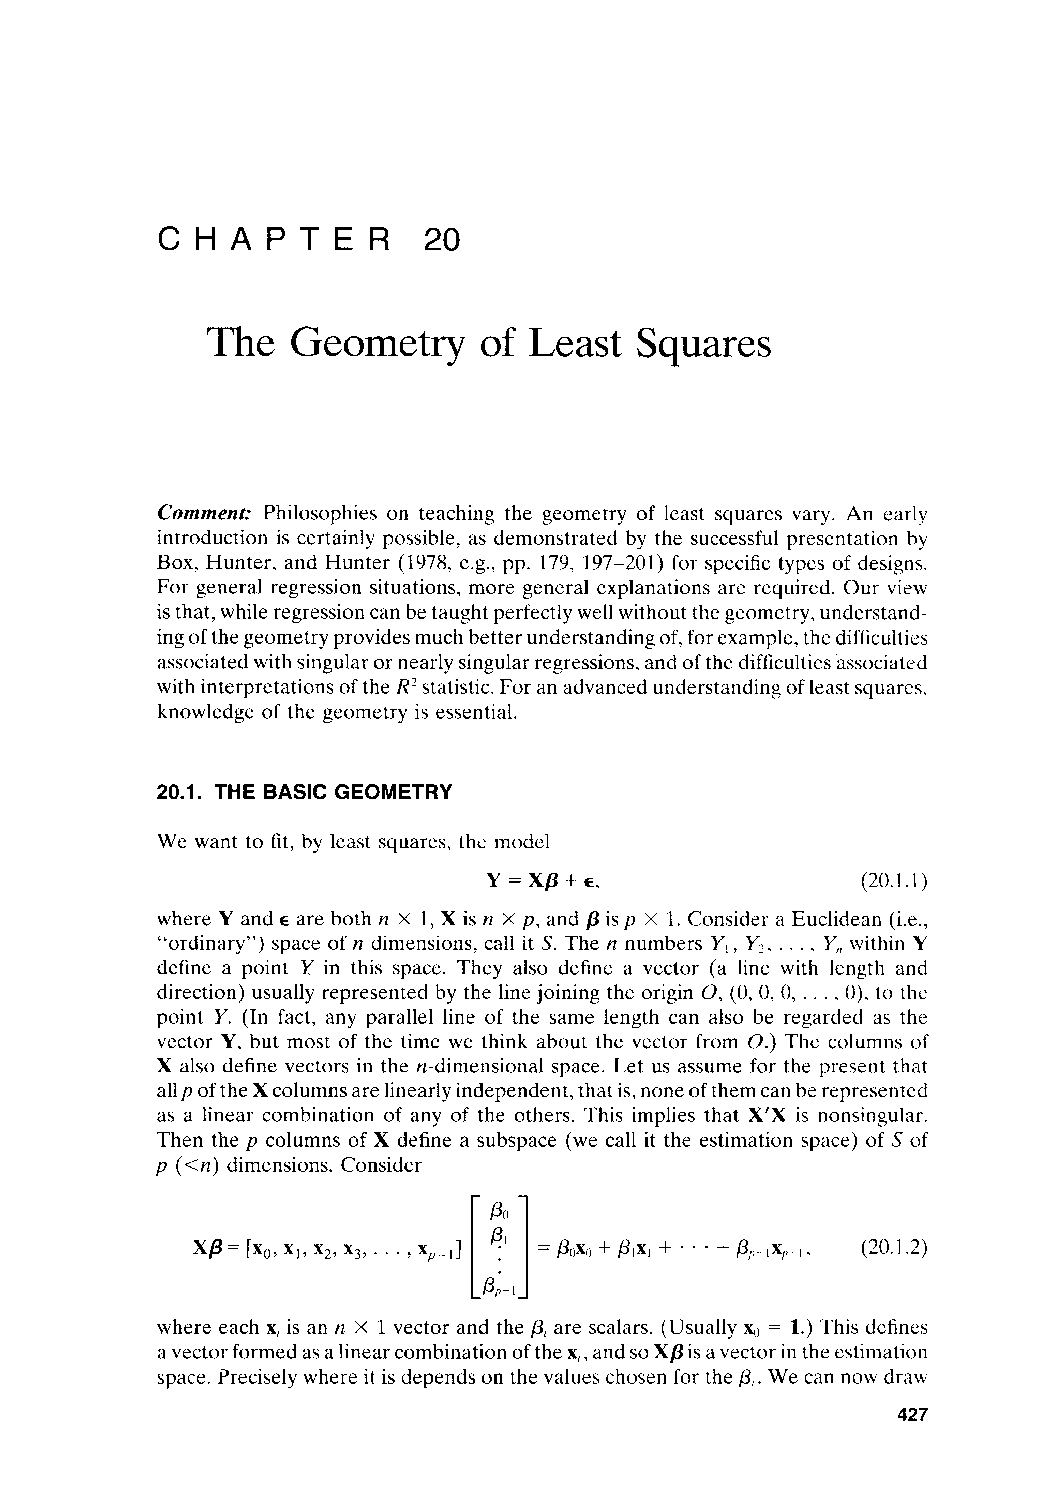
\includepdf[pages=-]{ch20.pdf}
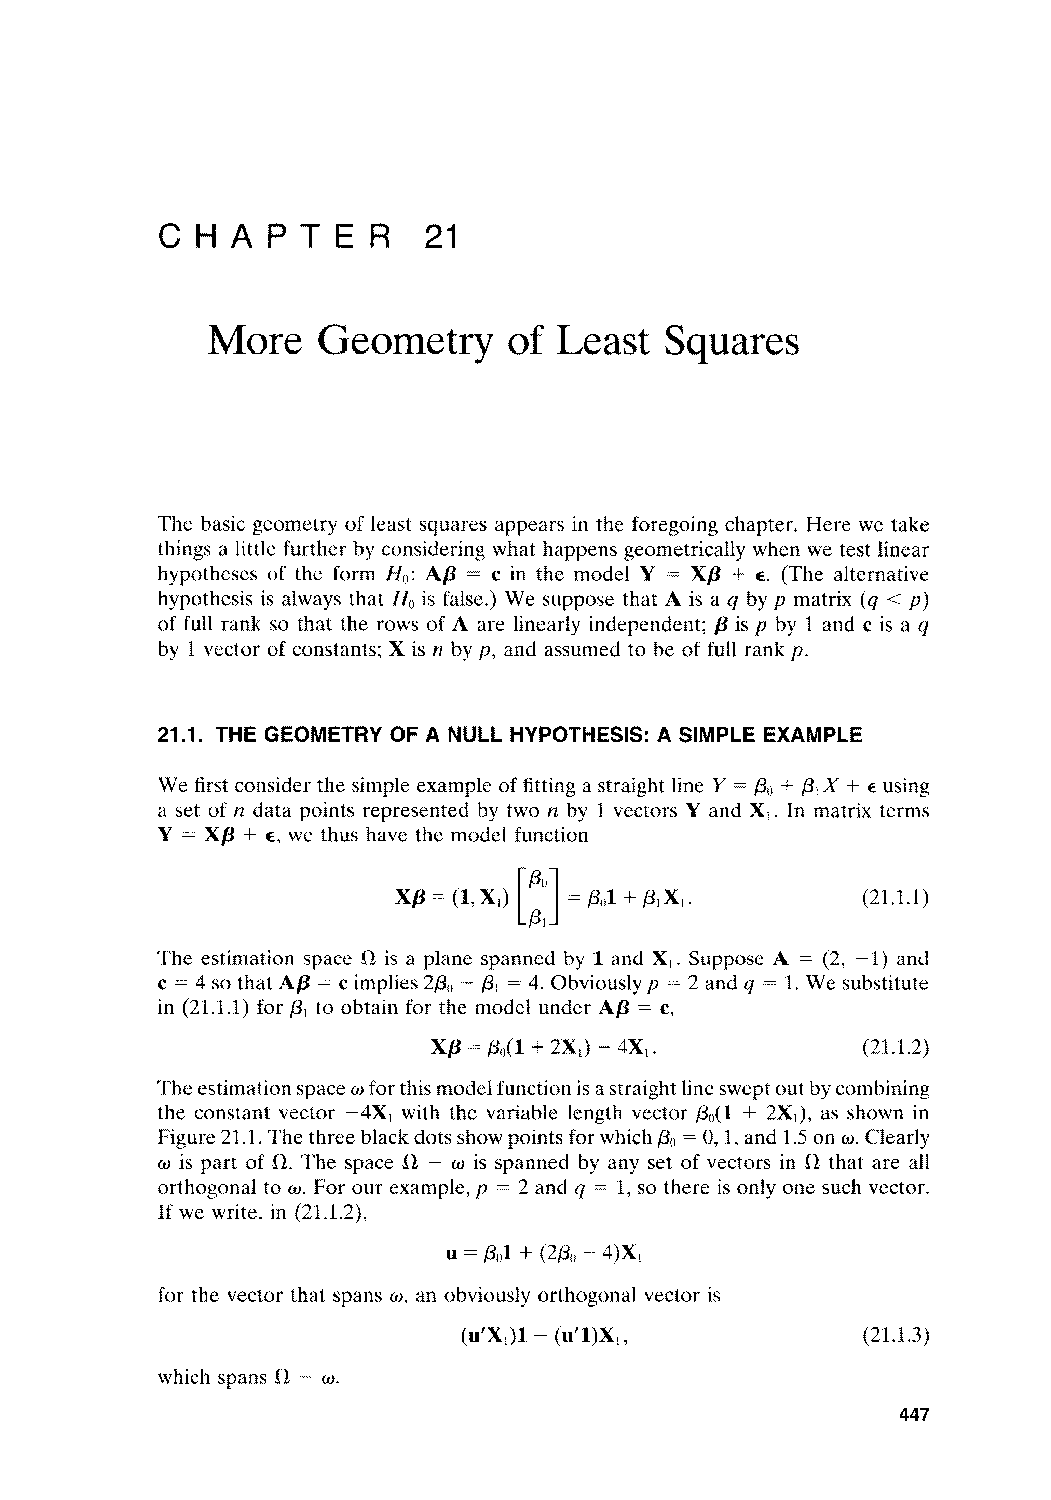
\includepdf[pages=-]{ch21.pdf}
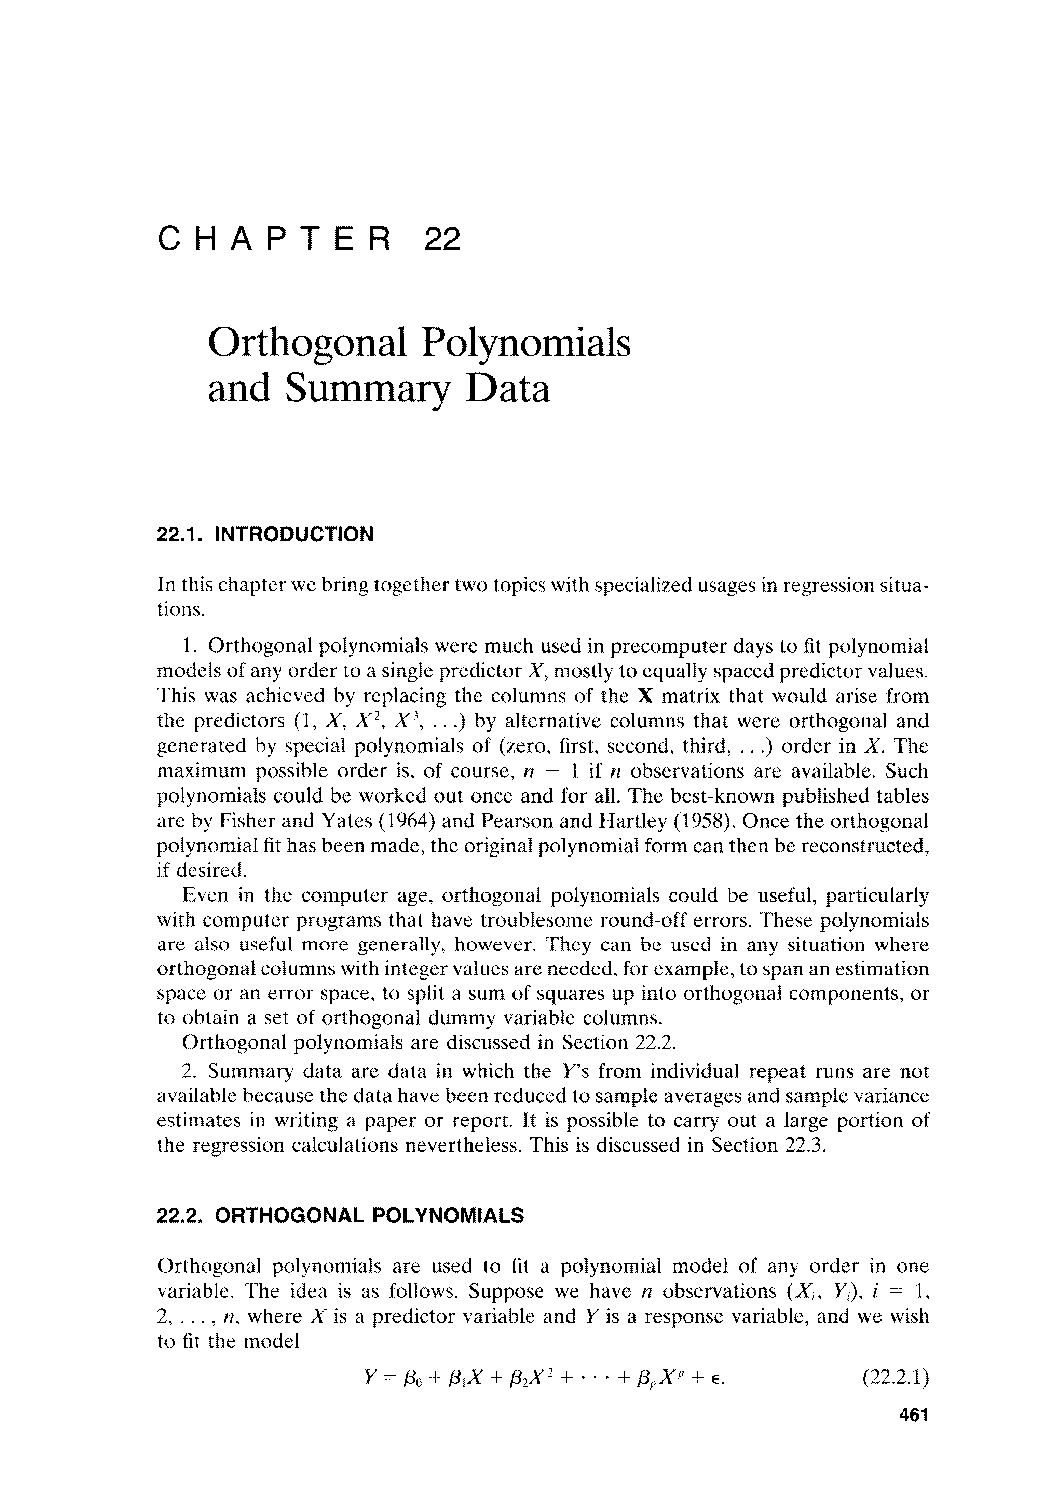
\includepdf[pages=-]{ch22.pdf}
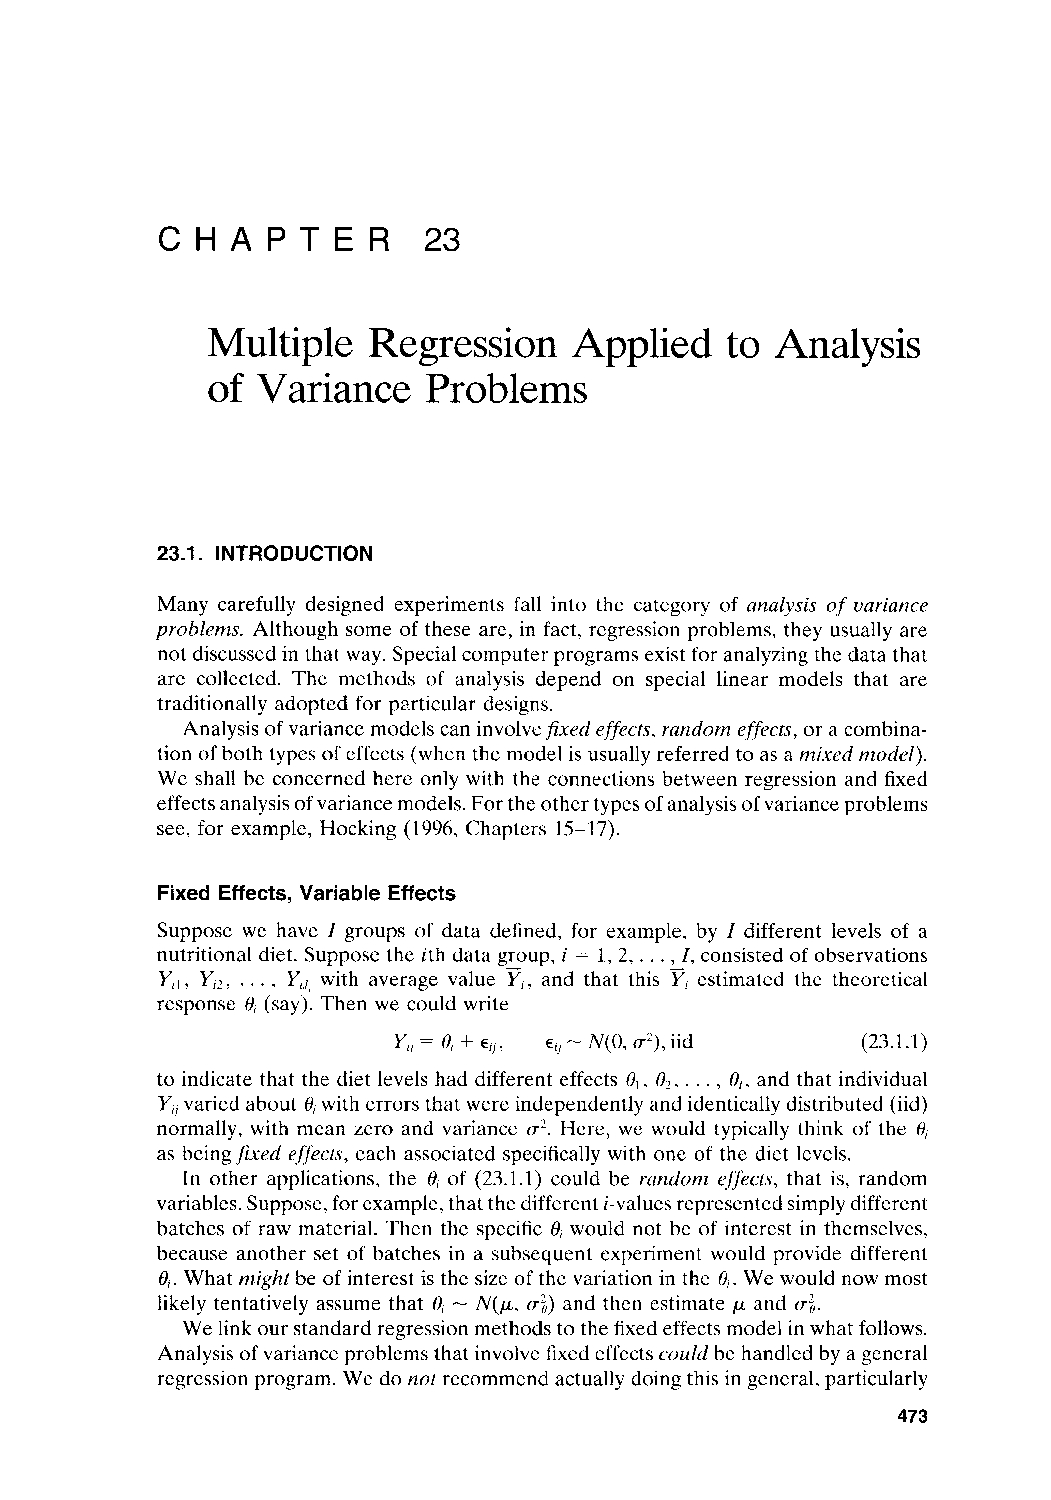
\includepdf[pages=-]{ch23.pdf}
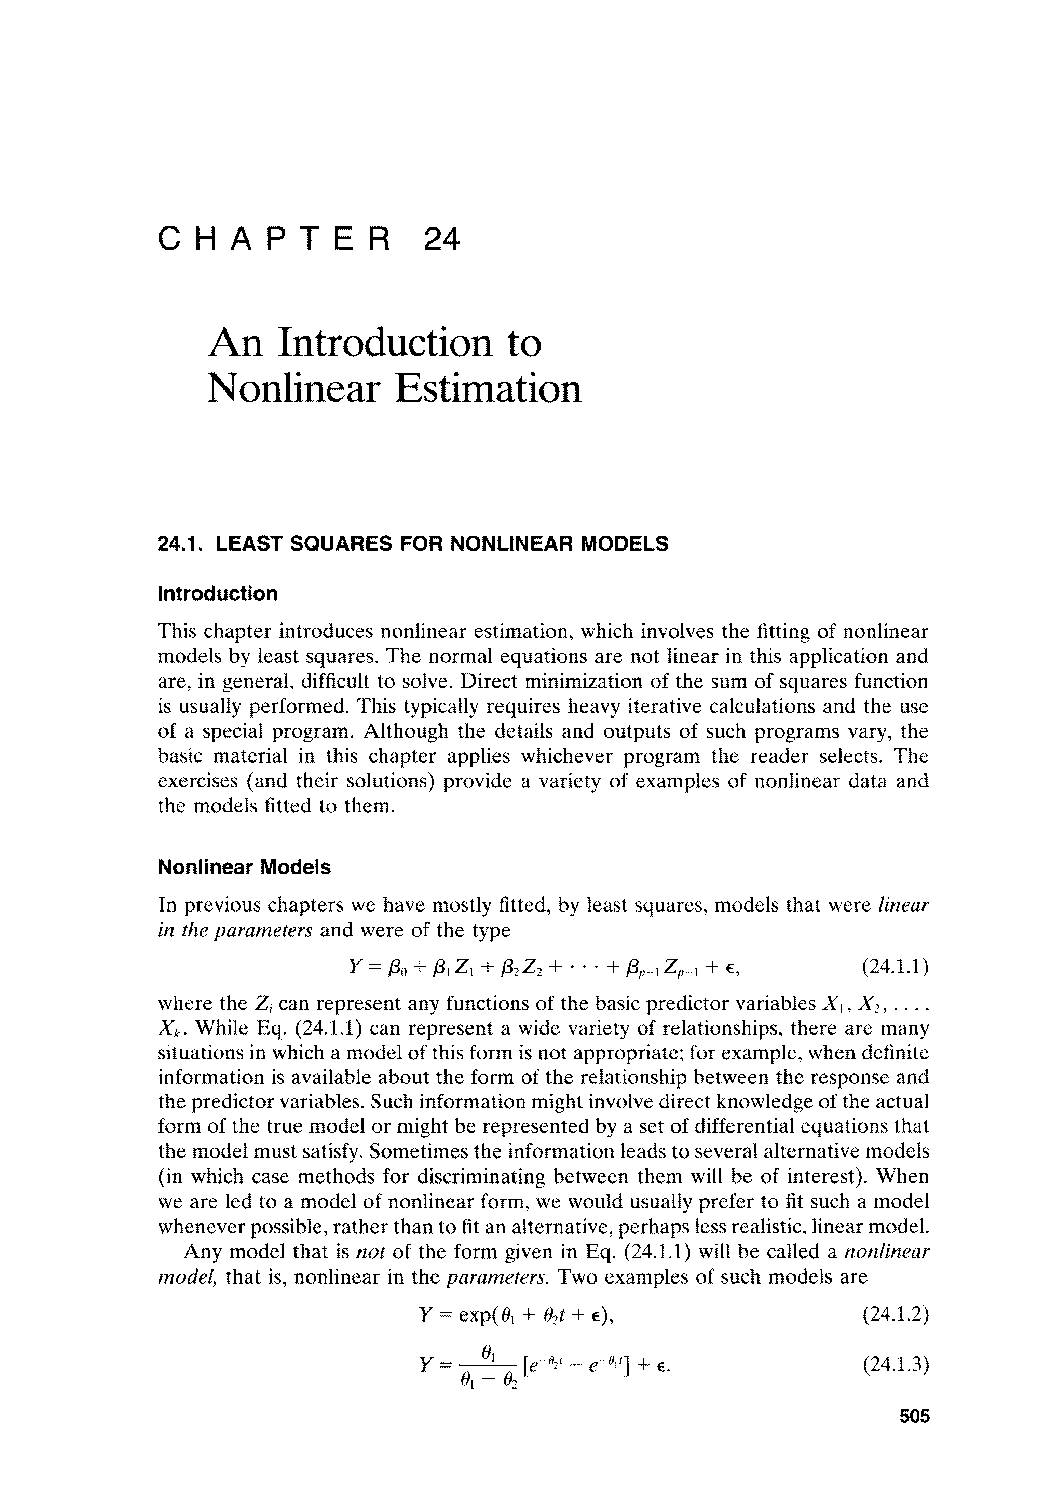
\includepdf[pages=-]{ch24.pdf}
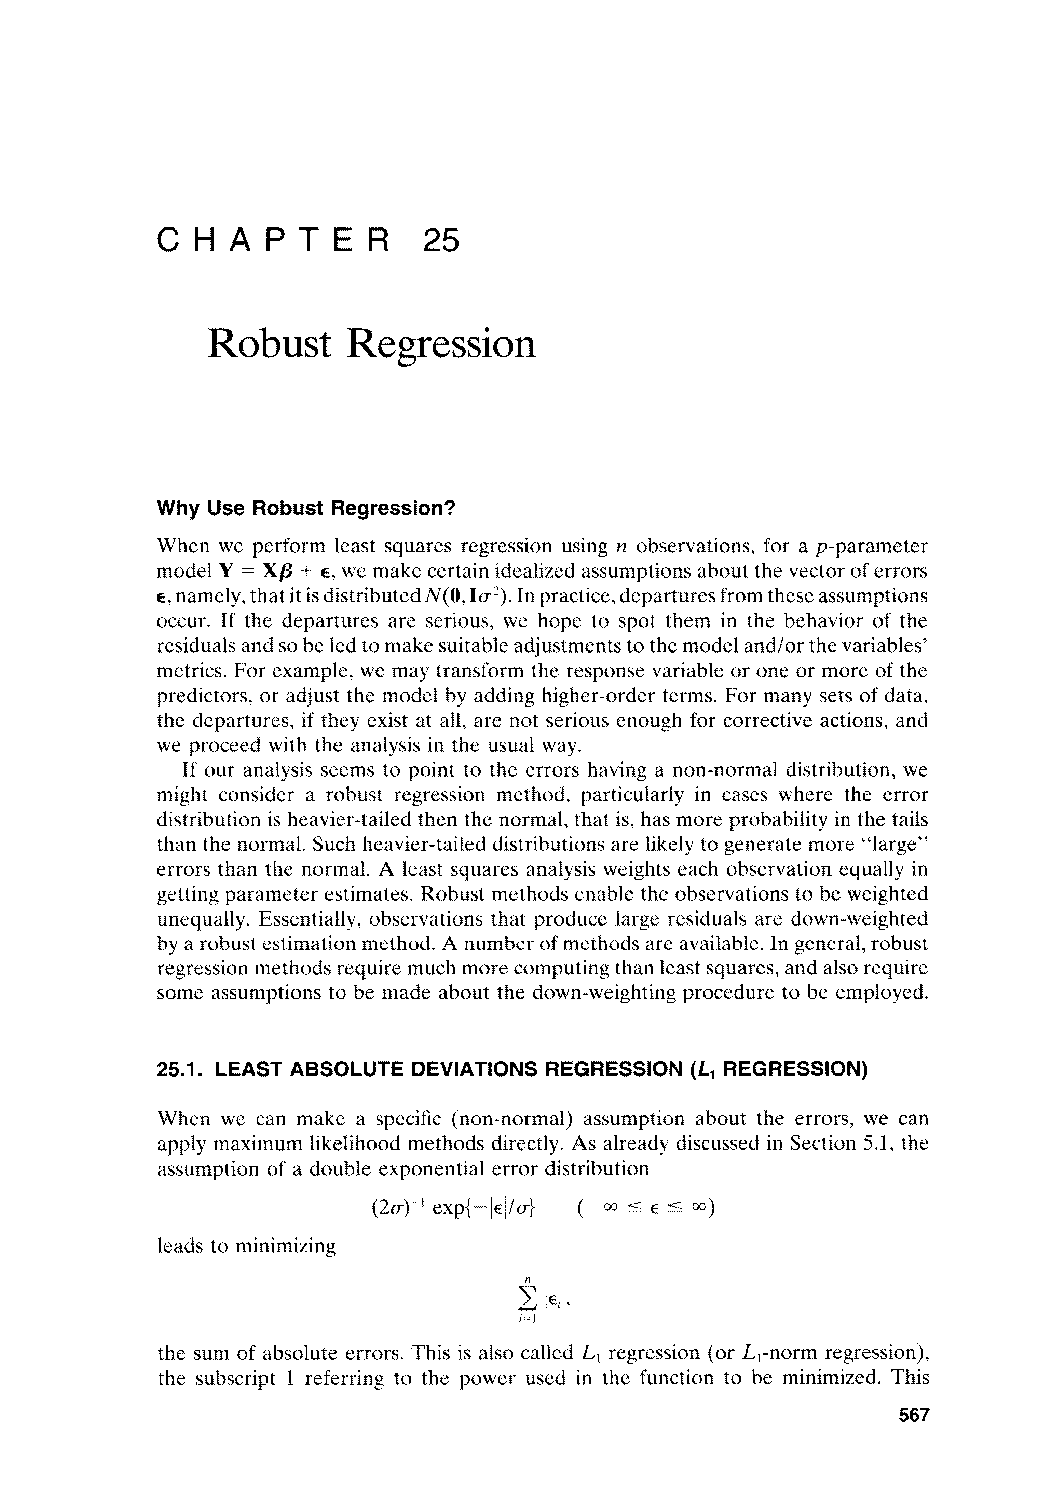
\includepdf[pages=-]{ch25.pdf}
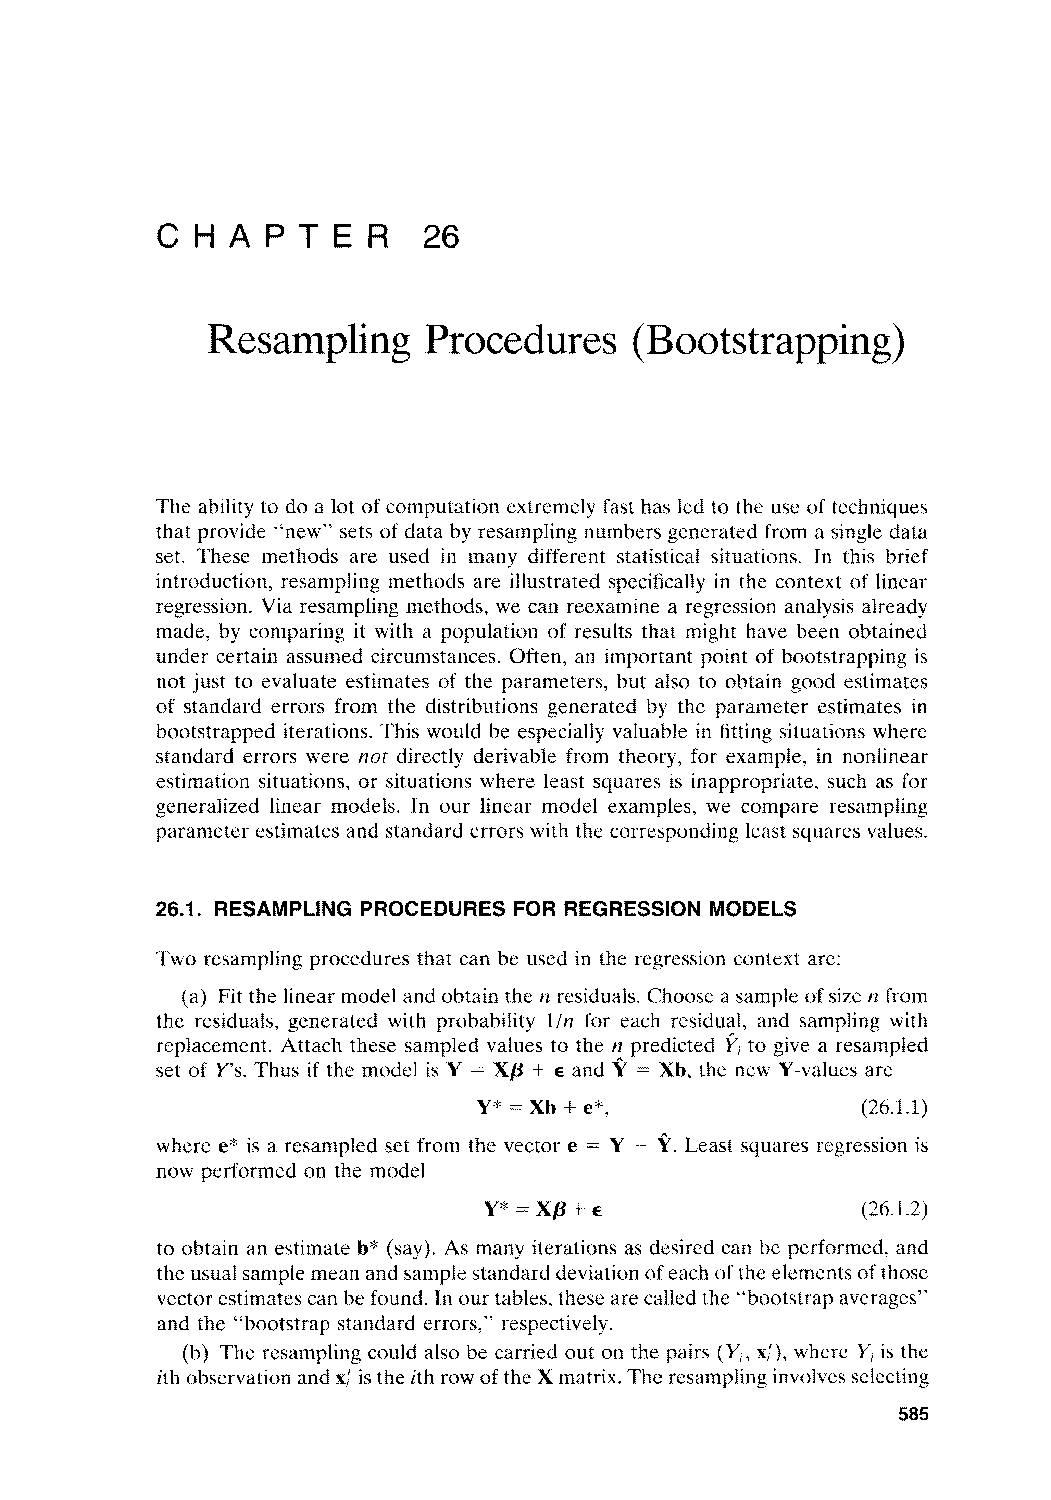
\includepdf[pages=-]{ch26.pdf}
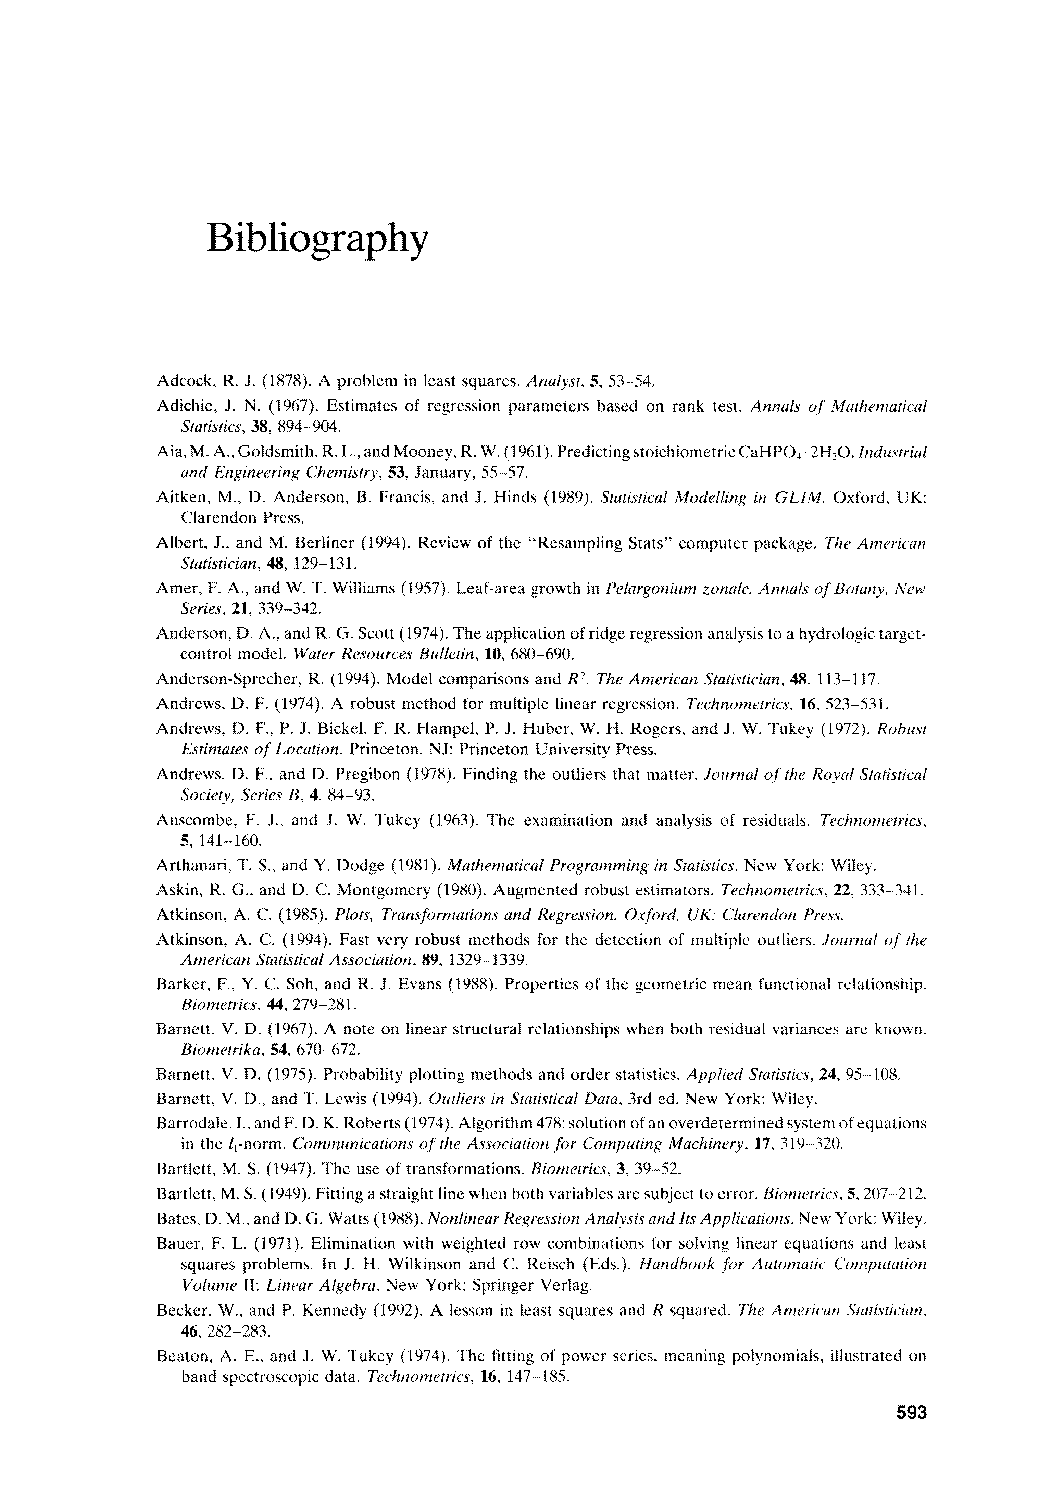
\includepdf[pages=-]{biblio.pdf}
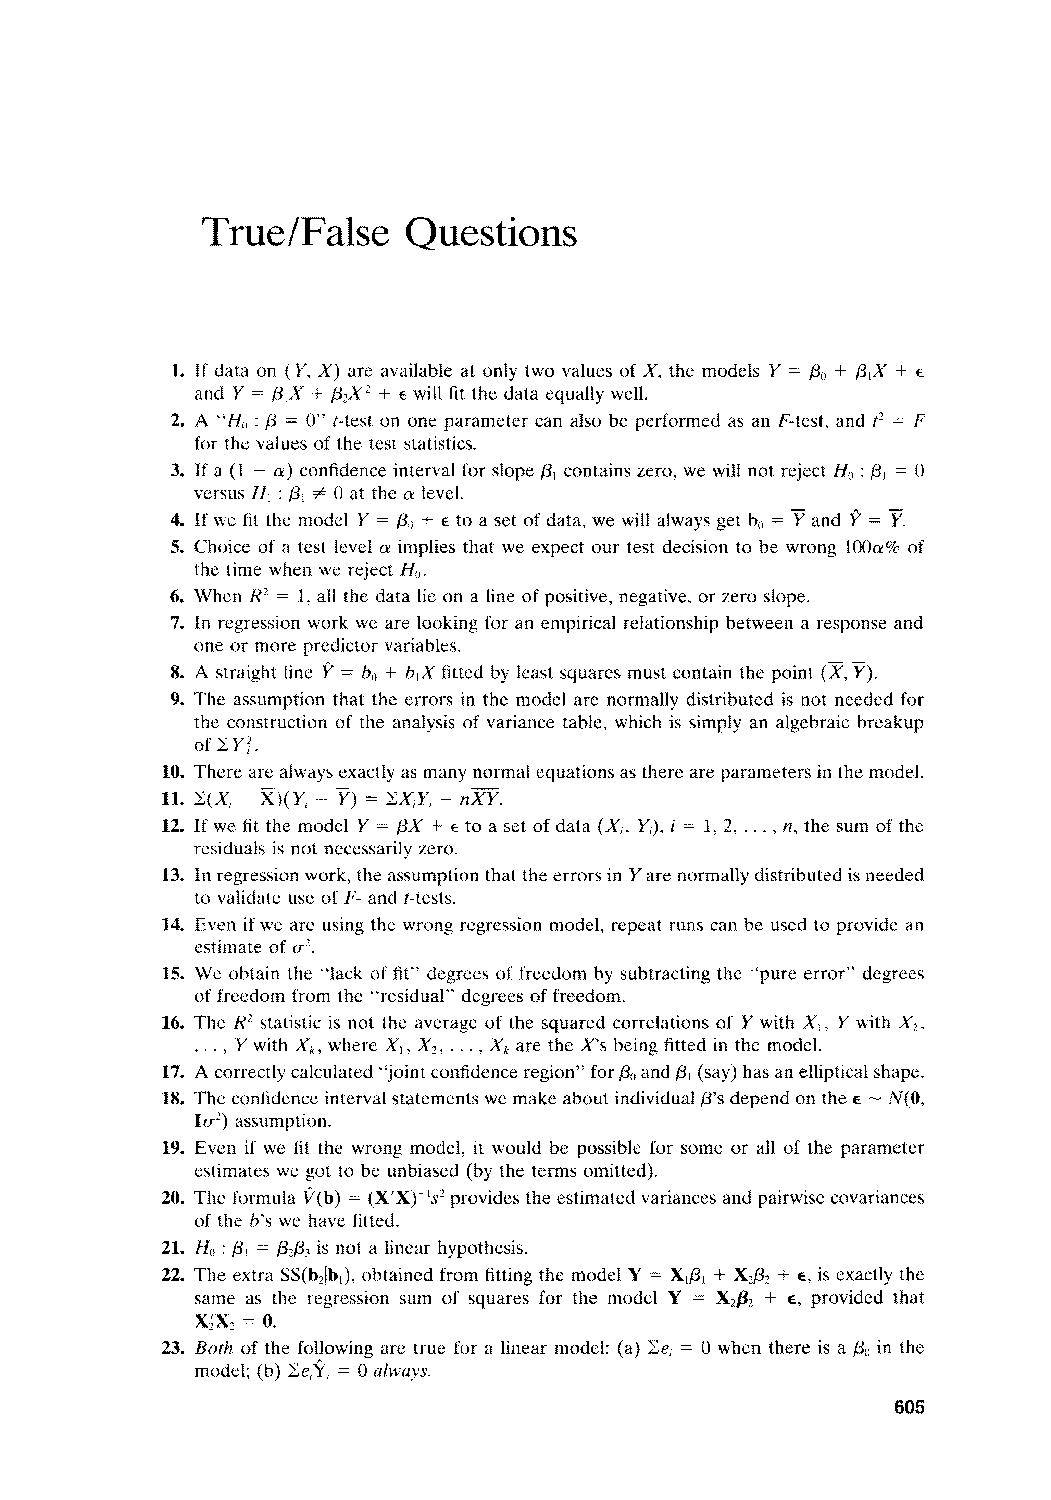
\includepdf[pages=-]{oth1.pdf}
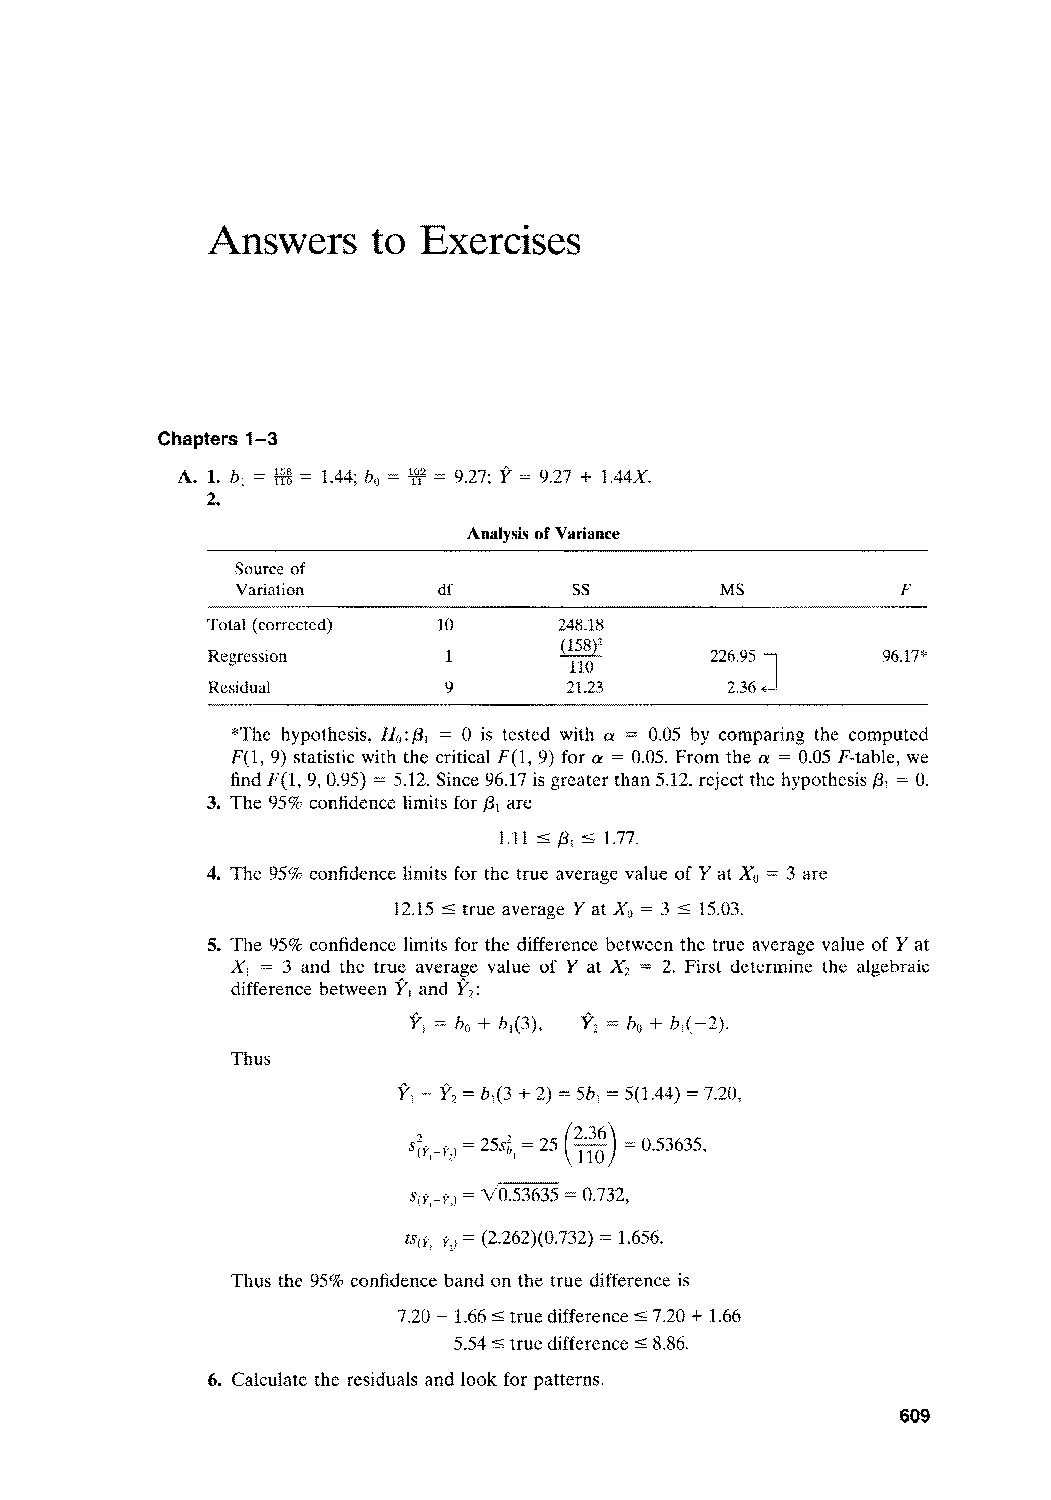
\includepdf[pages=-]{oth2.pdf}
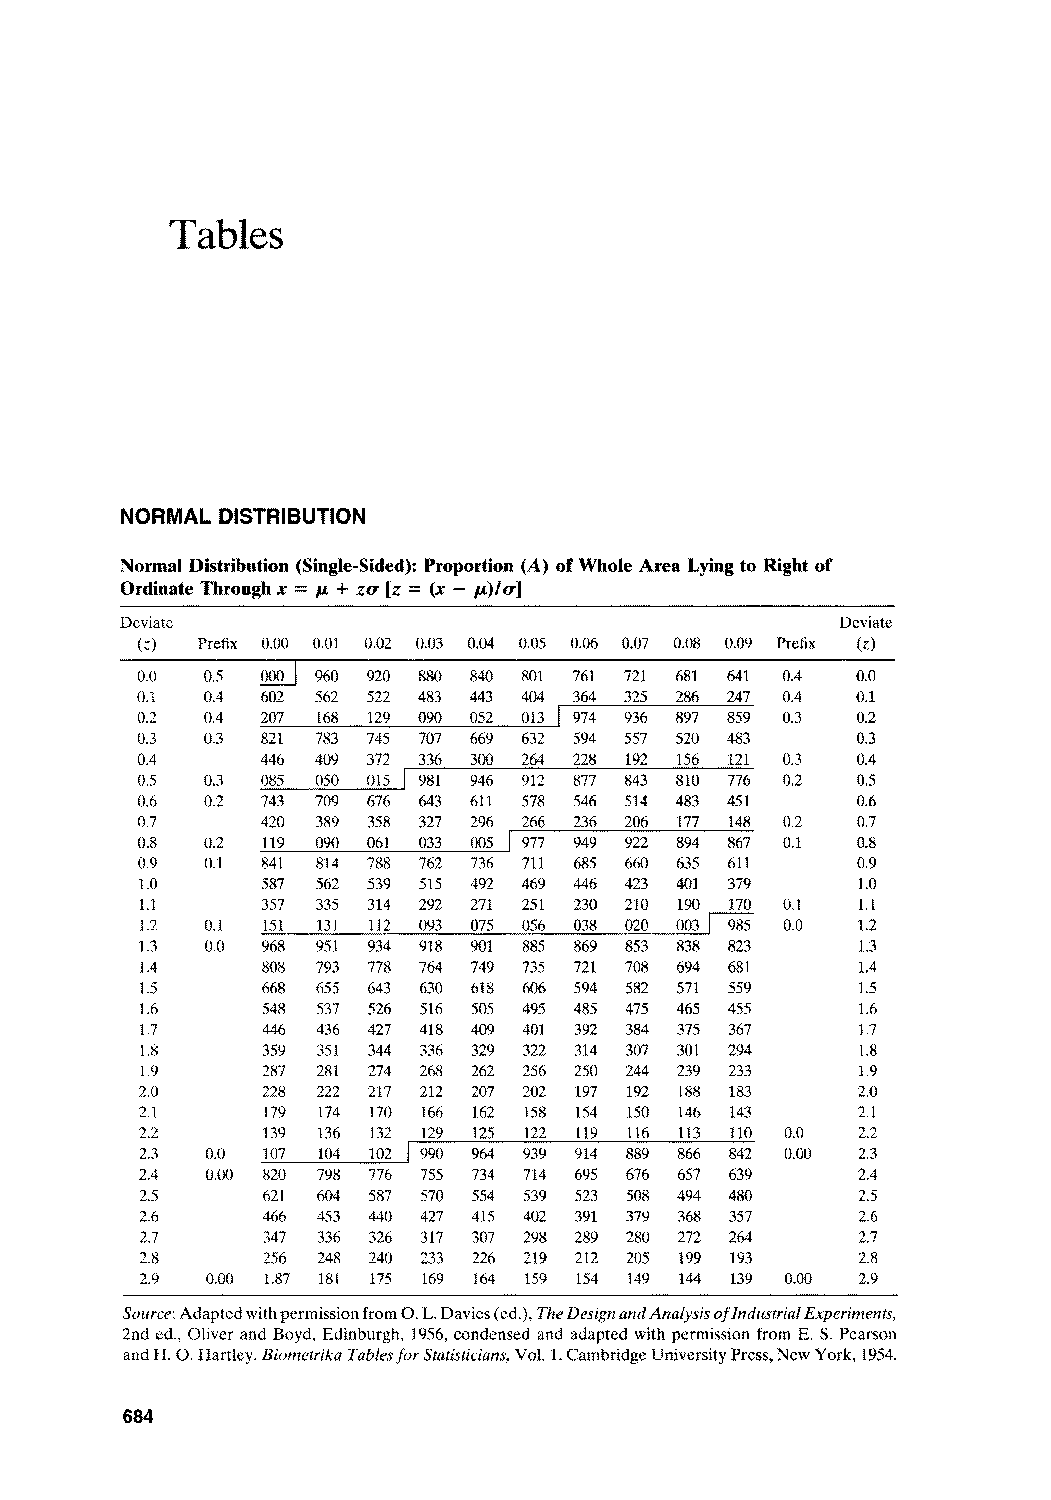
\includepdf[pages=-]{oth3.pdf}
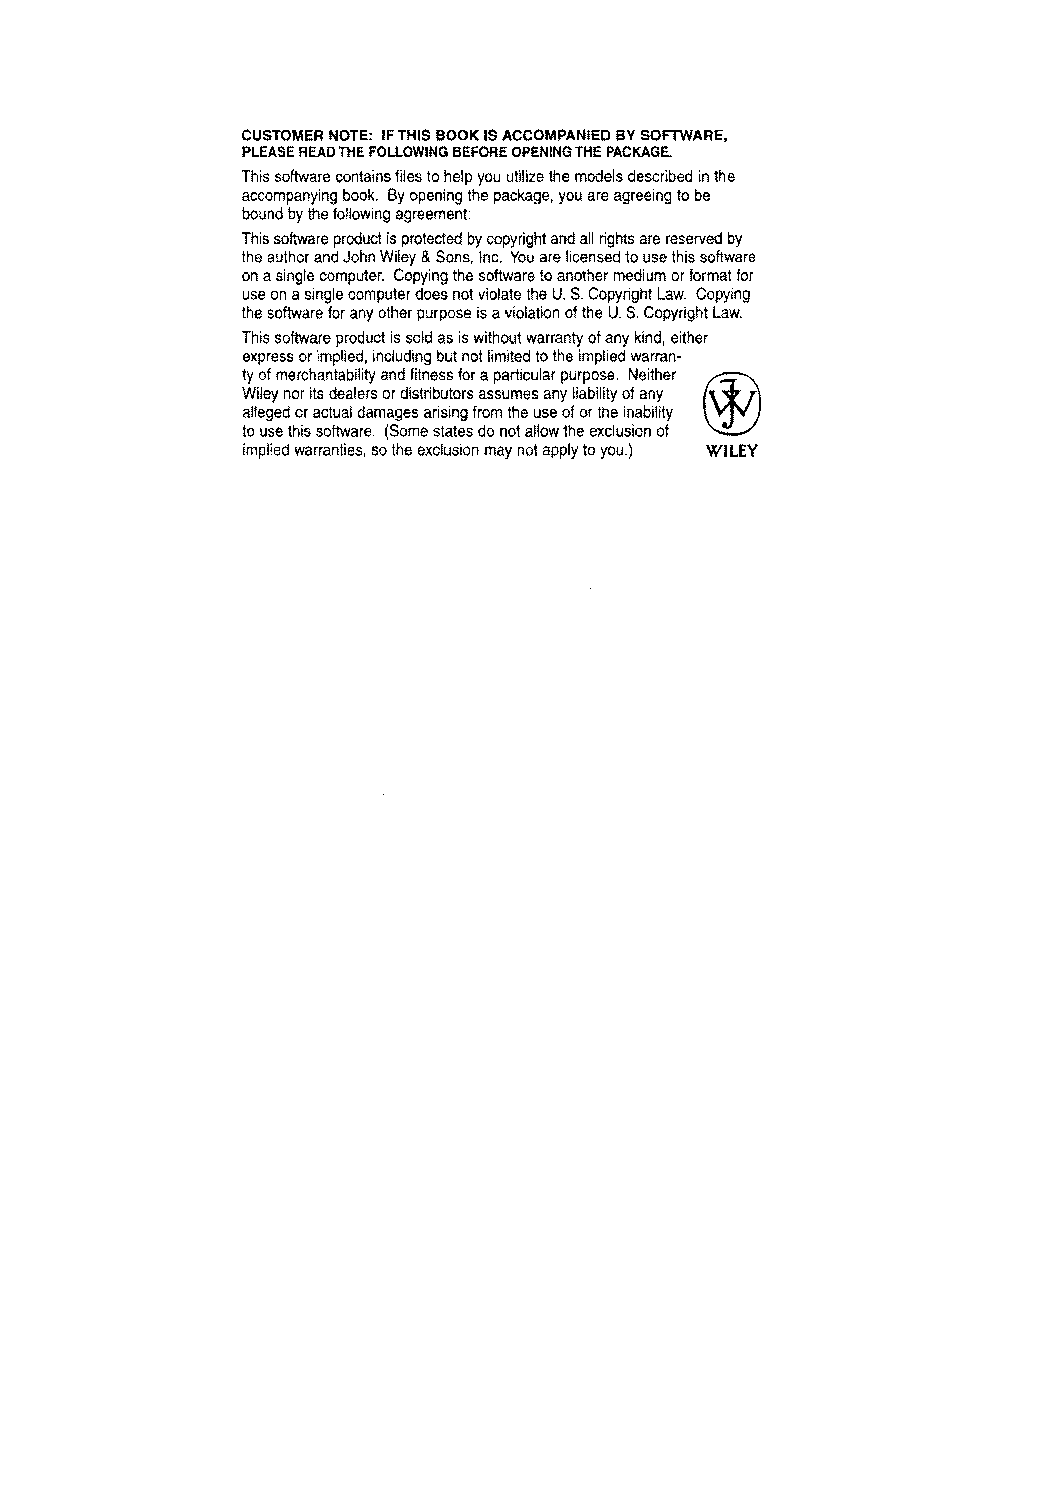
\includepdf[pages=-]{oth4.pdf}
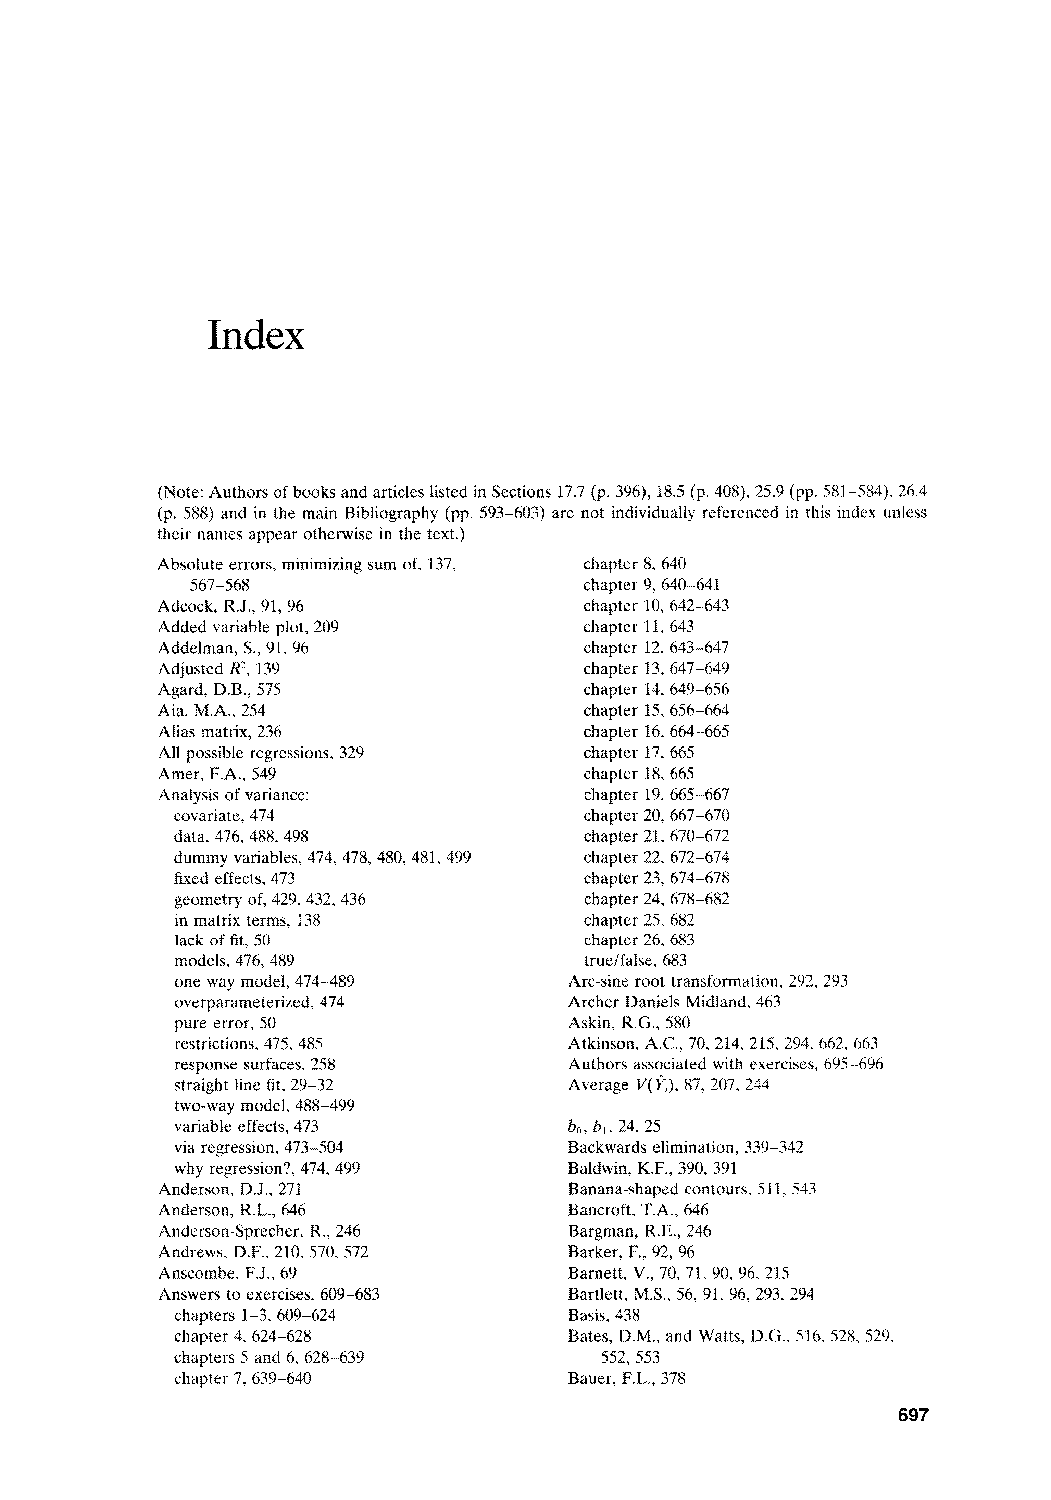
\includepdf[pages=-]{index.pdf}
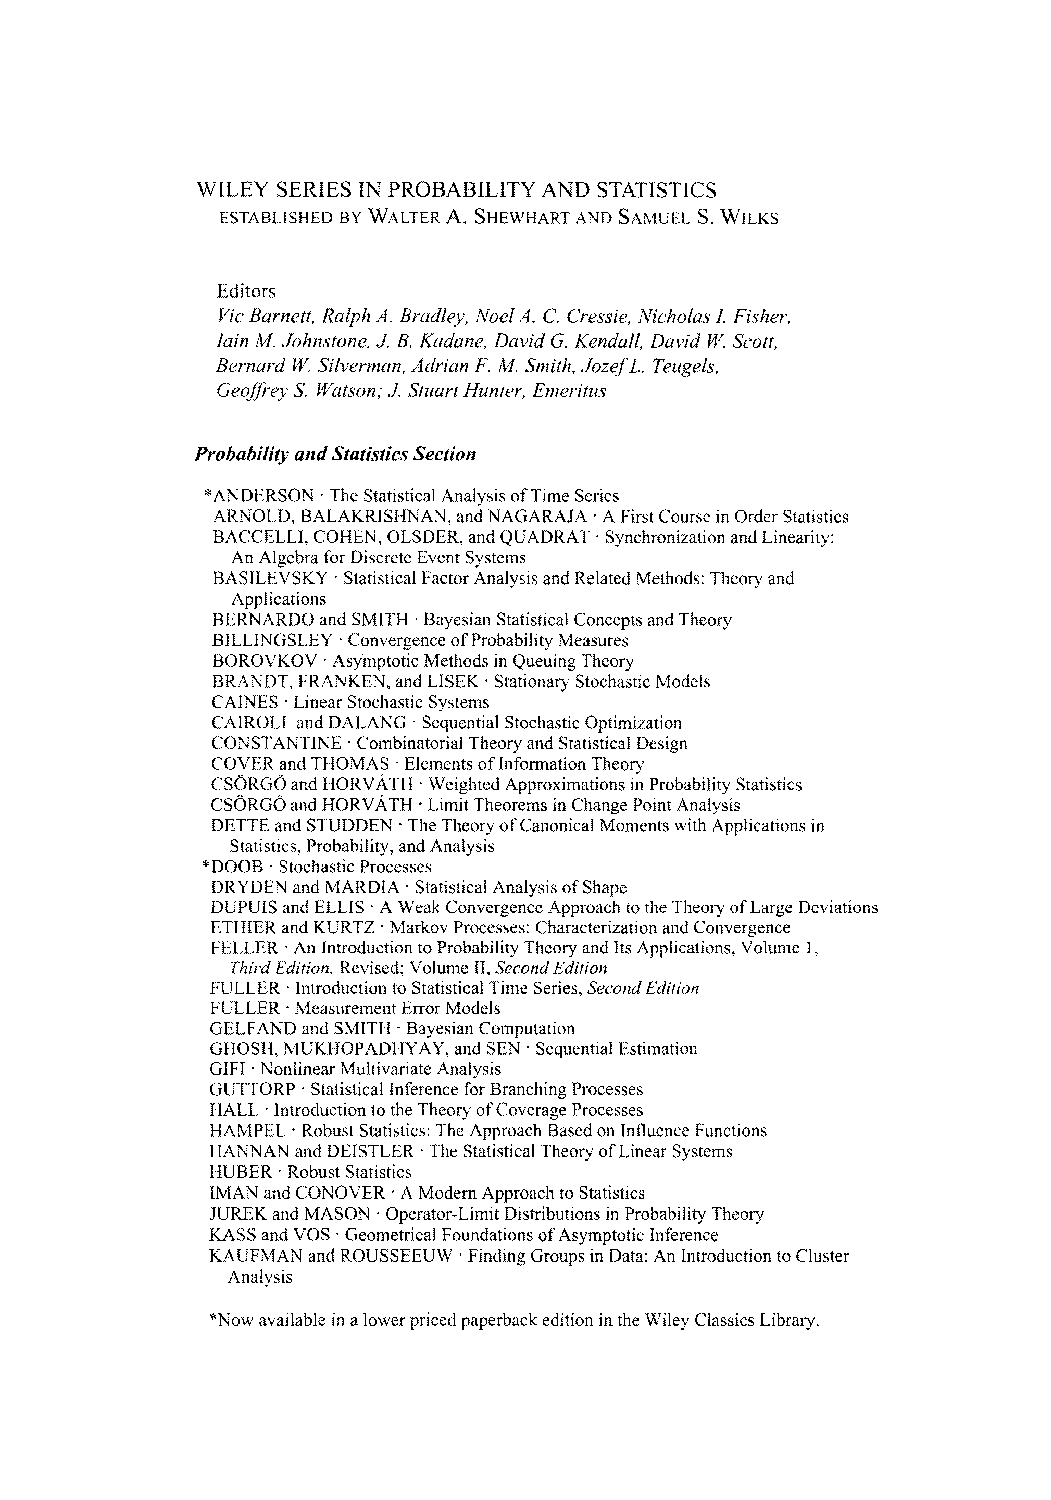
\includepdf[pages=-]{scard.pdf}
\end{document}